\documentclass[11pt]{article}

% Change "review" to "final" to generate the final (sometimes called camera-ready) version.
% Change to "preprint" to generate a non-anonymous version with page numbers.
\usepackage[review]{acl}

% Standard package includes
\usepackage{times}
\usepackage{latexsym}

% For proper rendering and hyphenation of words containing Latin characters (including in bib files)
\usepackage[T1]{fontenc}
% For Vietnamese characters
% \usepackage[T5]{fontenc}
% See https://www.latex-project.org/help/documentation/encguide.pdf for other character sets

% This assumes your files are encoded as UTF8
\usepackage[utf8]{inputenc}

% This is not strictly necessary, and may be commented out,
% but it will improve the layout of the manuscript,
% and will typically save some space.
\usepackage{microtype}

% This is also not strictly necessary, and may be commented out.
% However, it will improve the aesthetics of text in
% the typewriter font.
\usepackage{inconsolata}

%Including images in your LaTeX document requires adding
%additional package(s)
\usepackage{graphicx}
\usepackage{amsmath}
\usepackage{amssymb}
\usepackage{float}
\IfFileExists{placeins.sty}{
  \usepackage{placeins}
}{
  \newcommand{\FloatBarrier}{}
}
\IfFileExists{tcolorbox.sty}{
  \usepackage[most]{tcolorbox}
  \tcbuselibrary{breakable}
  \newtcolorbox{promptbox}[1]{
    enhanced jigsaw,
    breakable,
    parbox=false,
    colback=gray!8,
    colframe=gray!8,
    boxrule=0pt,
    arc=0.8mm,
    boxsep=0.3mm,
    left=0.7mm,
    right=0.7mm,
    top=0.5mm,
    bottom=0.5mm,
    before skip=1pt,
    after skip=1pt,
    pad at break*=0mm,
    fontupper=\scriptsize,
    before upper={\noindent\textbf{##1}\par\vspace{1pt}\raggedright\sloppy\setlength{\parskip}{0.5pt}\setlength{\parindent}{0pt}}
  }
  \newtcolorbox{promptcontbox}{
    enhanced jigsaw,
    breakable,
    parbox=false,
    colback=gray!8,
    colframe=gray!8,
    boxrule=0pt,
    arc=0.8mm,
    boxsep=0.3mm,
    left=0.7mm,
    right=0.7mm,
    top=0.5mm,
    bottom=0.5mm,
    before skip=0pt,
    after skip=1pt,
    pad at break*=0mm,
    fontupper=\scriptsize,
    before upper={\raggedright\sloppy\setlength{\parskip}{0.5pt}\setlength{\parindent}{0pt}}
  }
}{
  \newenvironment{promptbox}[1]{%
    \par\medskip
    \noindent\textbf{##1}\par
    \begingroup\scriptsize\noindent
  }{%
    \par\endgroup\medskip
  }
  \newenvironment{promptcontbox}{%
    \par
    \begingroup\scriptsize\noindent
  }{%
    \par\endgroup\medskip
  }
}

% Use a consistent ACL/EMNLP-style readable table font across the paper.
% Avoid globally redefining \scriptsize, since it makes appendix tables and prompt boxes harder to place.
% \let\scriptsize\small

% If the title and author information does not fit in the area allocated, uncomment the following
%
%\setlength\titlebox{<dim>}
%
% and set <dim> to something 5cm or larger.

\title{CA-Mem: Overcoming the Cross-Lingual Knowledge Bottleneck via Concept-Anchored Memory Agent}

% Author information can be set in various styles:
% For several authors from the same institution:
% \author{Author 1 \and ... \and Author n \\
%         Address line \\ ... \\ Address line}
% if the names do not fit well on one line use
%         Author 1 \\ {\bf Author 2} \\ ... \\ {\bf Author n} \\
% For authors from different institutions:
% \author{Author 1 \\ Address line \\  ... \\ Address line
%         \And  ... \And
%         Author n \\ Address line \\ ... \\ Address line}
% To start a separate ``row'' of authors use \AND, as in
% \author{Author 1 \\ Address line \\  ... \\ Address line
%         \AND
%         Author 2 \\ Address line \\ ... \\ Address line \And
%         Author 3 \\ Address line \\ ... \\ Address line}

\author{First Author \\
  Affiliation / Address line 1 \\
  Affiliation / Address line 2 \\
  Affiliation / Address line 3 \\
  \texttt{email@domain} \\\And
  Second Author \\
  Affiliation / Address line 1 \\
  Affiliation / Address line 2 \\
  Affiliation / Address line 3 \\
  \texttt{email@domain} \\}

%\author{
%  \textbf{First Author\textsuperscript{1}},
%  \textbf{Second Author\textsuperscript{1,2}},
%  \textbf{Third T. Author\textsuperscript{1}},
%  \textbf{Fourth Author\textsuperscript{1}},
%\\
%  \textbf{Fifth Author\textsuperscript{1,2}},
%  \textbf{Sixth Author\textsuperscript{1}},
%  \textbf{Seventh Author\textsuperscript{1}},
%  \textbf{Eighth Author \textsuperscript{1,2,3,4}},
%\\
%  \textbf{Ninth Author\textsuperscript{1}},
%  \textbf{Tenth Author\textsuperscript{1}},
%  \textbf{Eleventh E. Author\textsuperscript{1,2,3,4,5}},
%  \textbf{Twelfth Author\textsuperscript{1}},
%\\
%  \textbf{Thirteenth Author\textsuperscript{3}},
%  \textbf{Fourteenth F. Author\textsuperscript{2,4}},
%  \textbf{Fifteenth Author\textsuperscript{1}},
%  \textbf{Sixteenth Author\textsuperscript{1}},
%\\
%  \textbf{Seventeenth S. Author\textsuperscript{4,5}},
%  \textbf{Eighteenth Author\textsuperscript{3,4}},
%  \textbf{Nineteenth N. Author\textsuperscript{2,5}},
%  \textbf{Twentieth Author\textsuperscript{1}}
%\\
%\\
%  \textsuperscript{1}Affiliation 1,
%  \textsuperscript{2}Affiliation 2,
%  \textsuperscript{3}Affiliation 3,
%  \textsuperscript{4}Affiliation 4,
%  \textsuperscript{5}Affiliation 5
%\\
%  \small{
%    \textbf{Correspondence:} \href{mailto:email@domain}{email@domain}
%  }
%}

\begin{document}
\maketitle
\begin{abstract}
Large language models often degrade sharply when reasoning in low-resource languages.
We attribute this degradation to a cross-lingual knowledge bottleneck: fragile LRL surface representations do not reliably elicit knowledge associated with dense, high-resource language conceptual hubs.
Existing prompting and translation strategies either assume correct initial knowledge routing or preserve task-irrelevant surface details, which can amplify reasoning drift.
\textbf{CA-Mem} is a Concept-Anchored Memory Agent that separates multilingual reasoning into three stages.
First, \textit{Concept Anchoring} abstracts the LRL query into an HRL concept and boundary definition, providing a more stable semantic interface.
Second, CA-Mem retrieves from a curated \textit{Concept Usage Memory} that stores procedural heuristics distilled from source-side problem-solving trajectories rather than raw facts or full QA traces.
Third, the model answers the original query with both the concept anchor and the retrieved usage guidance.
On Global-MMLU, CA-Mem achieves 66.24 macro accuracy and improves over strong translation and structured-prompting baselines by more than 4 points. The gains further generalize to INCLUDE and MGSM, as well as across Qwen, Llama, Ministral, and Gemma, suggesting that concept-anchored procedural memory provides an effective interface in the evaluated low-resource multilingual reasoning settings.
\end{abstract}

\section{Introduction}

Large language models (LLMs) demonstrate strong reasoning and knowledge-acquisition capabilities, yet they still degrade substantially when applied to low-resource languages (LRLs) \citep{qin2024does,zhang2025survey}.
This discrepancy is closely related to the imbalanced distribution of pre-training corpora.
High-resource languages (HRLs), such as English, provide much denser training signals, allowing LLMs to form more stable latent concept representations.
In contrast, sparse exposure to LRLs can produce less reliable representations that fail to align with these established conceptual hubs \citep{zhu2024multilingual,cao2024exploring}.
% Consequently, while the requisite knowledge already resides within the model's parameters, LRL inputs struggle to reliably activate it.
We follow prior work in referring to this as the cross-lingual knowledge bottleneck \citep{goworek2025bridging}: LRL queries may trigger unstable routing paths in latent space, causing reasoning failures before downstream inference can use the relevant knowledge.

To address this bottleneck, conventional approaches primarily rely on prompt formatting or surface-level language conversion.
Reasoning enhancement techniques, such as Chain-of-Thought (CoT) \citep{wei2022chain} and its structured variants \citep{qi2025sot}, enforce step-by-step generation.
However, they lack mechanisms to ensure correct initial concept activation; if the model misroutes the LRL query at the outset, structural prompting may simply elaborate an incorrect trajectory \citep{chen2025halumem}.
Alternatively, translation-based strategies, such as Translate-Test~\citep{etxaniz2024multilingual} or Self-Translate~\citep{liu2025translation}, attempt to bypass the LRL barrier by converting the entire prompt into an HRL.
While this can mitigate surface-level comprehension issues, holistic translation may preserve task-irrelevant details and noisy distractors.
It fails to explicitly decouple and highlight the core concepts required for problem-solving, leaving the model vulnerable to reasoning drift and context interference.

Recent work explores memory-augmented agents that provide external knowledge or historical reasoning trajectories \citep{liu2025agent0,zhang2026g}.
MemoryBank \citep{zhong2024memorybank}, A-Mem \citep{xu2026mem}, and Mem0 \citep{chhikara2025mem0} utilize Retrieval-Augmented Generation (RAG) pipelines to fetch relevant past interactions or factual paragraphs.
Despite their success in monolingual or HRL settings, applying these memory systems directly to LRL reasoning introduces new challenges.
First, querying a memory bank using raw LRL text or its direct translation can suffer from cross-lingual representation mismatch, leading to noisy or redundant similarity retrieval \citep{hu2026beyond}.
Second, retrieving raw factual texts or complete historical QA pairs merely provides declarative context.
It does not directly equip the model with the procedural knowledge of \textit{how} to apply a specific concept under complex constraints, and it can exacerbate lost-in-the-middle effects or token inefficiency \citep{liu2026simplemem}.

To tackle these challenges, we propose CA-Mem, a framework that shifts from passive text retrieval to explicit conceptual alignment and procedural experience reuse.
Our approach operates via a three-stage mechanism.
First, the agent executes concept anchoring, where it abstracts the raw LRL query into a concise HRL concept name and its boundary definition.
Second, using this explicit concept anchor, the agent retrieves from a curated concept usage memory.
Third, the agent conducts memory-augmented reasoning by combining the original query, the activated concept-description pair, and the retrieved usage memory.
Instead of storing raw texts, this memory retains procedural summaries of how specific concepts were successfully applied in source-side examples.
Experiments on multiple multilingual benchmarks across diverse LLMs show that our framework consistently outperforms competitive translation and structural baselines.
In summary, our main contributions are as follows:
\begin{itemize}
    \item We propose the concept-anchored memory agent framework.
    By explicitly generating HRL concepts and definitions, we align fragile LRL inputs into a stable, high-resource concept space, improving conceptual routing.
    \item We introduce the concept usage memory to store and retrieve procedural problem-solving experiences rather than declarative texts.
    \item We empirically show that providing concept-aligned usage experience improves multilingual reasoning and generalizes across multiple LLM families.
\end{itemize}

%%%%%%%%%%%%%%%%%%%%%%%%%%%%%%%%%%%%%%%%%%%%%%%%%%%%%%%%%%%%%%%%%%%%%%%%%%%%%%%%%
\section{Related Work}

\textbf{Low-Resource Multilingual Reasoning}
LLM reasoning capabilities remain skewed toward HRLs \citep{huang2023not,zhu2024multilingual}, causing large performance drops on LRL benchmarks \citep{shi2022language,ponti2020xcopa}.
Representation analyses suggest that LRL inputs often map to less stable regions in latent space, making them harder to align with HRL concept hubs \citep{cao2024exploring,tang2024language}.
Consequently, an important bottleneck in LRL reasoning is knowledge elicitation rather than only knowledge absence \citep{qin2024does}.
Our work addresses this bottleneck by explicitly mapping fragile LRL inputs into a high-resource concept space before reasoning.

\begin{figure*}[t]
\centering
\IfFileExists{figures/framework.pdf}{
    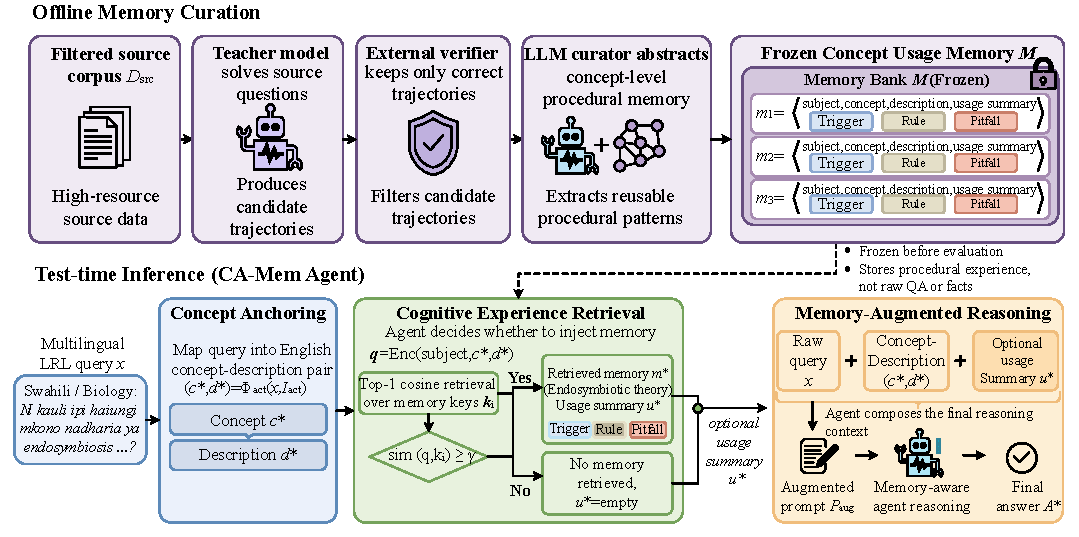
\includegraphics[width=0.98\textwidth]{figures/framework.pdf}
}{
    \fbox{
    \begin{minipage}[c][0.28\textheight][c]{0.92\textwidth}
    \centering
    Figure 1 placeholder: overall architecture of CA-Mem.\\
    Concept Anchoring $\rightarrow$ Concept Usage Memory Retrieval $\rightarrow$ Memory-Augmented Reasoning.
    \end{minipage}
    }
}
\caption{\textbf{CA-Mem}. The agent first anchors a multilingual input into an English concept-description pair, retrieves concept-aligned procedural memory, and then performs memory-augmented reasoning.}
\label{fig:framework}
\end{figure*}

\textbf{Translation and Prompting Methods}
Training-free interventions typically mitigate LRL deficits through language conversion or reasoning formatting.
Conversion strategies, such as English-centric reasoning~\citep{etxaniz2024multilingual} and Self-Translate~\citep{liu2025translation}, map LRL queries to English before inference.
However, as demonstrated by \citet{liu2025translation}, holistic translation can preserve surface-level noise and task-irrelevant distractors, failing to isolate the core concepts necessary for deduction.
Alternatively, prompting paradigms like CoT \citep{wei2022chain} and SoT \citep{qi2025sot} enforce step-by-step rationales.
Recent multilingual reasoning studies also show that models can generate English rationales for non-English questions, motivating cross-lingual CoT-style baselines \citep{ranaldi2025natural}.
Yet, these methods implicitly assume correct initial knowledge routing.
If an LRL input activates the wrong concept, structural prompting can elaborate an already-misaligned trajectory \citep{chen2025halumem}.
Our Concept Anchoring operates orthogonally: it abstracts the LRL input into a concise HRL concept definition before any structural reasoning is applied.

\textbf{Retrieval and Memory-Augmented Reasoning}
RAG fetches external contexts to reduce hallucinations \citep{gao2023retrieval}, but applying RAG to LRLs suffers from cross-lingual representation mismatch, yielding noisy and redundant contexts \citep{zhang2025survey}.
To improve retrieval efficiency, agent memory systems structure historical interactions \citep{zhong2024memorybank, chhikara2025mem0}.
Recent architectural optimizations, such as SimpleMem \citep{liu2026simplemem} and Beyond RAG \citep{hu2026beyond}, decouple and compress episodic traces to prevent similarity collapse.
Despite these structural advances, existing memories predominantly retrieve declarative facts or raw historical states.
They lack the procedural heuristics required to apply specific concepts to novel scenarios \citep{kim2024rada}.
Building upon hierarchical memory distillation, we introduce the concept usage memory.
Instead of caching declarative texts, our memory stores abstract, procedural usage experiences.
Retrieving these experiential guidelines via anchored HRL concepts reduces cross-lingual mismatch and injects procedural knowledge for LRL reasoning.

%%%%%%%%%%%%%%%%%%%%%%%%%%%%%%%%%%%%%%%%%%%%%%%%%%%%%%%%%%%%%%%%%%%%%%%%%%%%%%%%%%
\section{Methodology}


% \begin{figure*}[t]
%     \centering
%     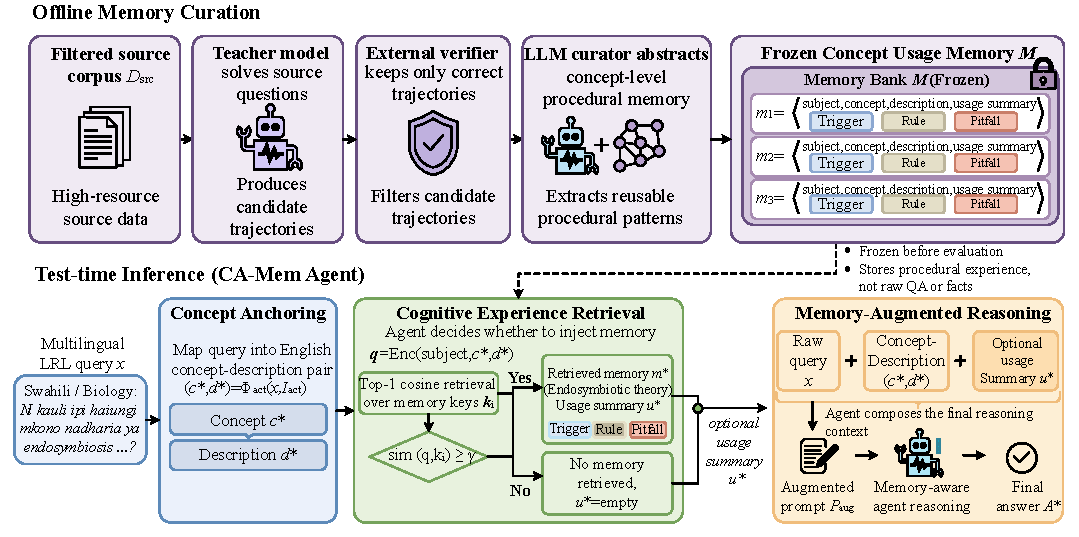
\includegraphics[scale =0.5]{figures/framework.pdf}
%     \caption{The overall architecture of the Concept-Anchored Memory Agent.}
%     \label{fig:overall_framework}
% \end{figure*}

We propose CA-Mem, a structured framework designed to mitigate the cross-lingual knowledge bottleneck in LLMs.
Rather than relying on fragile surface-level predictions from LRLs, CA-Mem decomposes inference into three sequential phases: Concept Anchoring, Cognitive Experience Retrieval, and Memory-Augmented Reasoning.
As illustrated in Figure~\ref{fig:framework}, the agent first abstracts the raw LRL query into an HRL conceptual representation, uses this semantic anchor to retrieve relevant procedural experiences from a frozen memory bank, and then combines these elements to predict the final answer.


\subsection{Concept Anchoring for Cross-Lingual Elicitation}

Directly prompting an LLM with an LRL query $x$ can force reasoning from a sparse and less reliable representation, leading to knowledge elicitation failures.
To address this, Concept Anchoring projects the LRL input onto a denser HRL conceptual interface before deduction.
Given an activation instruction $\mathcal{I}_{\mathrm{act}}$, the agent decodes an HRL conceptual tuple $z = (c, d)$, where $c$ is the core concept name and $d$ is its boundary definition.
Rather than performing an intractable joint search over the concept and description spaces, we enforce a directed dependency during inference.
We obtain the tuple with sequential greedy decoding (temperature $\tau=0$):

\begin{align}
    c^* &= \operatorname*{arg\,max}_{c} P_\theta(c \mid x, \mathcal{I}_{\mathrm{act}}) \\
    d^* &= \operatorname*{arg\,max}_{d} P_\theta(d \mid x, \mathcal{I}_{\mathrm{act}}, c^*)
\end{align}
This autoregressive factorization makes $c^*$ an explicit semantic anchor, while the subsequent description $d^*$ bounds its interpretive scope.
This mapping reduces LRL-specific surface noise and stabilizes the initial reasoning context.

\subsection{Concept Usage Memory}
To bridge the gap between concept identification and execution, we introduce the Concept Usage Memory, a structured repository designed to encode and supply procedural heuristics.

\subsubsection{Memory Node Representation}

Unlike standard RAG paradigms that cache declarative facts or raw question-answer pairs, our architecture isolates procedural knowledge.
We formalize the memory bank as a set of structured nodes $\mathcal{M} = \{m_1, m_2, \dots, m_K\}$.
Each node $m_i$ is instantiated as a heterogeneous tuple:

\begin{equation}
    m_i = \langle s_i, c_i, d_i, u_i \rangle
\end{equation}
where $s_i \in \mathcal{S}$ represents the subject or domain constraint, $c_i \in \mathcal{C}$ denotes the semantic concept anchor, $d_i \in \mathcal{D}$ defines the precise conceptual boundary, and $u_i \in \mathcal{U}$ is the core usage summary.
The usage summary $u_i$ fundamentally distinguishes our approach from traditional memory stores.
Rather than preserving specific factual states, $u_i$ encodes the generalized procedural heuristics governing the application of $c_i$.
We treat $u_i$ as a compact set of constraints that guide the downstream reasoning function.
Specifically, $u_i = \{ \omega_{\mathrm{trig}}, \omega_{\mathrm{rule}}, \omega_{\mathrm{err}} \}$ contains trigger invariants, decision rules, and negative error boundaries (i.e., common pitfalls), respectively.
By retrieving $u_i$, the agent acquires explicit instructions on how to operationalize the anchored concept within the targeted domain $s_i$.

\subsubsection{Offline Memory Curation}

% To ensure the external memory bank provides high-quality, generalizable procedural experiences without introducing evaluation bias, we strictly decouple the memory construction phase from the downstream inference environment.
% The offline memory bank $\mathcal{M}$ is curated from an independent source-side corpus $\mathbb{D}_{\mathrm{src}}$.
% To prevent data leakage, we remove any source question that is exactly identical to a test question before either SFT construction or memory building.
% The remaining source pool is then used as the shared basis for both CA-SFT data and offline memory curation.
% Subsequently, a teacher model solves source-side questions from the filtered pool and produces solving trajectories.
% We only curate memory from verifier-approved trajectories, where the teacher prediction is judged correct by an external verifier.
% The source-side gold label is used only for eligibility verification and is not stored in the memory node or provided to the curator as reusable memory content.
% A curator policy then abstracts these verified trajectories into stable concept-level procedural memory nodes.
% To ensure $u_i$ captures transferable procedural knowledge rather than overfitting to specific instance details, the curation process is optimized following the Information Bottleneck principle.
% Given a set of historical trajectories $\mathcal{T}_{c_i}$ associated with concept $c_i$, the optimal usage summary $u_i^*$ maximizes the mutual information with the generalized solving logic $Y$ while penalizing the retention of instance-specific surface variables $X$:
% \begin{equation}
% \small
%     u_i^* = \mathop{\arg\max}_{u \in \mathcal{U}} \Big[ I(u; Y \mid c_i, \mathcal{T}_{c_i}) - \beta I(u; X \mid c_i, \mathcal{T}_{c_i}) \Big]
% \end{equation}
% where $\beta$ controls the compression rate, ensuring $u_i^*$ abstracts purely procedural rules.
% Once curated, the memory bank $\mathcal{M}$ remains strictly frozen during the entire downstream evaluation phase.
% The test queries only perform retrieval against $\mathcal{M}$, guaranteeing that the observed performance gains stem entirely from the zero-shot transfer of concept-aligned usage experience, rather than trivial test-set caching or continual parameter updates.

To provide generalizable procedural experiences without introducing evaluation bias, the offline memory bank $\mathcal{M}$ is curated from a decontaminated source corpus filtered against the evaluation benchmarks, denoted $\mathcal{D}_{\mathrm{src}}$.
Candidate memory nodes originate from verifier-approved solving trajectories. 
To prevent the memory from overfitting to surface variables (e.g., instance-specific entities or numbers), we distill raw historical trajectories $\mathcal{T}_{c_i}$ into generalized usage summaries $u_i$.
Conceptually, this distillation is motivated by the Information Bottleneck (IB) principle: retaining information relevant to general solving logic while minimizing instance-specific details.
Because our curator is a frozen LLM $\Phi_{\mathrm{curate}}$ operating zero-shot, we do not explicitly optimize a parameterized mutual information objective.
Instead, we operationalize this compression-relevance trade-off through constrained prompt abstraction:

\begin{equation}
    u_i = \Phi_{\mathrm{curate}}(\mathcal{T}_{c_i} \mid \Omega_{\mathrm{IB}})
\end{equation}
where $\Omega_{\mathrm{IB}}$ represents the explicit instruction constraints that mandate the removal of specific instance details and the retention of purely procedural heuristics (trigger invariants, decision rules, and error boundaries).
Once curated, $\mathcal{M}$ remains entirely frozen during evaluation. 
Test queries only execute read operations, so downstream gains reflect zero-shot transfer of concept-aligned procedural knowledge under our filtering protocol rather than test-set updates.

\subsection{Memory-Augmented Retrieval and Reasoning}

After constructing a conceptual anchor and an offline procedural memory bank, the framework integrates these elements at inference time.
This design avoids direct retrieval with raw LRL queries, which can suffer from cross-lingual representation mismatch.
Inference therefore proceeds through Cognitive Experience Retrieval followed by Memory-Augmented Reasoning.

\subsubsection{Cognitive Experience Retrieval}

To fetch procedural heuristics, we implement a concept-based retrieval mechanism.
The retrieval query concatenates the domain subject $s$, the generated concept $c^*$, and the generated description $d^*$, isolating retrieval from the syntactic noise of the original LRL input $x$.
Let $\mathcal{E}_\phi: \mathcal{V}^* \rightarrow \mathbb{R}^d$ denote a dense embedding encoder. We formulate the retrieval query vector $\mathbf{q} \in \mathbb{R}^d$ as the encoded representation of the concatenated conceptual anchor:

\begin{equation}
    \mathbf{q} = \mathcal{E}_\phi \big( \mathrm{concat}(s, c^*, d^*) \big)
\end{equation}
Similarly, for each candidate node $m_i \in \mathcal{M}$, we compute a key vector $\mathbf{k}_i = \mathcal{E}_\phi \big( \mathrm{concat}(s_i, c_i, d_i) \big)$.
The relevance of a memory node is quantified via cosine similarity $S_{\mathrm{cos}}(\mathbf{q}, \mathbf{k}_i)$.
To reduce the injection of irrelevant or mismatched procedural memory, we enforce a gated retrieval strategy.
The top-ranked memory node is used only when its similarity exceeds a predefined confidence threshold $\gamma$. The retrieved memory $m^*$ is defined as:

\begin{equation}
    \hat{i} = \mathop{\arg\max}_{i \in \{1,\dots,K\}} S_{\mathrm{cos}}(\mathbf{q}, \mathbf{k}_i)
\end{equation}
\begin{equation}
    m^* =
    \begin{cases}
      m_{\hat{i}}, & \text{if } S_{\mathrm{cos}}(\mathbf{q}, \mathbf{k}_{\hat{i}}) \ge \gamma \\
      \emptyset, & \text{otherwise}
    \end{cases}
\end{equation}
When $m^* = \emptyset$, the framework defaults to the base concept-anchored setting without external memory injection.
This thresholding mechanism acts as a semantic filter, keeping the injected procedural heuristic $u^*$ closely aligned with the activated concept $c^*$.

\subsubsection{Memory-Augmented Reasoning}

% In the final reasoning phase, the LLM synthesizes the original context with the elicited HRL concepts and the retrieved procedural experience.
% We construct the augmented prompt context $\mathcal{P}_{\mathrm{aug}}$ by concatenating the raw LRL input $x$, the conceptual tuple $(c^*, d^*)$, and the retrieved usage summary $u^*$ (if $m^* \neq \emptyset$).
% The generation of the final answer $A$ is modeled as a conditional probability distribution over the augmented context.
% Formally, the language model parameterized by $\theta$ computes the optimal reasoning trajectory and final answer $A^*$ by maximizing the likelihood:

% \begin{equation}
%     A^* = \mathop{\arg\max}_{A} \prod_{t=1}^{|A|} P_\theta \big( a_t \mid x, c^*, d^*, u^*, a_{<t} \big)
% \end{equation}
% where $a_t$ represents the $t$-th token of the answer sequence.
% From an information-theoretic perspective, directly decoding from the LRL input $x$ yields a high-entropy prediction space $\mathcal{H}(A \mid x)$ due to the sparse activation of relevant latent knowledge.
% By explicitly conditioning the autoregressive generation on $c^*$ and $u^*$, we introduce strong deterministic priors.
% The conceptual anchor $c^*$ aligns the decoding process with the stable $\mathcal{M}_{\mathrm{HRL}}$ manifold, while the usage summary $u^*$ acts as a procedural regularizer, heavily penalizing decoding paths that violate established rule sets or boundary conditions.
% Consequently, the conditional entropy of the prediction space is strictly bounded:

% \begin{equation}
%     \mathcal{H}(A \mid x, c^*, d^*, u^*) \ll \mathcal{H}(A \mid x)
% \end{equation}
% This reduction in hypothesis space uncertainty is expected to reduce reasoning drift and conceptual misapplication, a pattern that we empirically examine in Section~\ref{sec:results}.

In the final reasoning phase, the agent synthesizes the raw LRL input $x$, the activated conceptual tuple $(c^*, d^*)$, and the retrieved usage summary $u^*$ (if $m^* \neq \emptyset$). 
The final answer $A^*$ is decoded by maximizing the conditional likelihood:

\begin{equation}
    A^* = \mathop{\arg\max}_{A} \prod_{t=1}^{|A|} P_\theta \big( a_t \mid x, c^*, d^*, u^*, a_{<t} \big)
\end{equation}
Directly decoding from a sparse LRL input yields a highly uncertain prediction space. 
By conditioning generation on $c^*$ and $u^*$, we introduce explicit priors.
From an information-theoretic perspective, informative conditioning can reduce the effective prediction space when the added variables are relevant.
Practically, the concept $c^*$ aligns decoding with the stable HRL manifold, while $u^*$ acts as a procedural regularizer that penalizes rule violations. 
This conditioning can reduce reasoning drift and conceptual misapplication during execution.

%%%%%%%%%%%%%%%%%%%%%%%%%%%%%%%%%%%%%%%%%%%%%%%%%%%%%%%%%%%%%%%%%%%%%%%%%%%%%%%%%
\section{Experiments}

We evaluate CA-Mem on three multilingual benchmarks: Global-MMLU~\citep{singh2025global}, INCLUDE~\citep{romanou2025include}, and MGSM~\citep{shi2022language}. For Global-MMLU, we report per-language accuracy and Macro Avg. on bn, sw, te, ne, and hi. For INCLUDE, we report per-language accuracy and Weighted Avg. on bn, te, ne, and hi because language-specific test sizes differ. For MGSM, we report per-language accuracy and Macro Avg. on bn, sw, and te. Appendix~\ref{sec:app_dataset} provides detailed language counts, including the English and Chinese auxiliary splits.

\begin{table*}[t]
\centering
\scriptsize
\setlength{\tabcolsep}{2.2pt}
\renewcommand{\arraystretch}{0.90}
\begin{tabular*}{\textwidth}{@{\extracolsep{\fill}} c l c c c c c c}
\hline
Model & Method & bn & sw & te & ne & hi & Macro Avg. \\
\hline
 & Zero-shot & 52.50 & 52.86 & 43.14 & 48.58 & 54.14 & 50.24 \\
 & CoT & 54.02 & 54.09 & 44.71 & 50.40 & 55.54 & 51.75 \\
 & Cross-CoT & 55.10 & 54.58 & 45.20 & 51.48 & 56.51 & 52.57 \\
Base & Self-Translate & 55.60 & 54.66 & 45.55 & 51.42 & 56.23 & 52.69 \\
 & SoT & 55.96 & 54.85 & 45.75 & 51.97 & 57.26 & 53.16 \\
 & CA-only & 56.67 & 56.00 & 46.08 & 52.81 & 57.80 & 53.87 \\
 & CA-Mem & \textbf{60.77} & \textbf{60.37} & \textbf{50.10} & \textbf{56.83} & \textbf{61.66} & \textbf{57.95} \\
\cline{1-8}
 & Zero-shot & 55.23 & 52.51 & 48.39 & 52.21 & 56.47 & 52.96 \\
 & CoT & 57.54 & 54.87 & 51.50 & 54.65 & 58.58 & 55.43 \\
 & Cross-CoT & 58.42 & 56.10 & 52.98 & 56.10 & 60.12 & 56.74 \\
Direct-SFT & Self-Translate & 59.17 & 56.95 & 53.55 & 57.26 & 60.75 & 57.54 \\
 & SoT & 57.59 & 55.00 & 51.49 & 55.24 & 58.91 & 55.65 \\
 & CA-only & 60.68 & 57.62 & 53.67 & 57.81 & 61.65 & 58.29 \\
 & CA-Mem & \textbf{65.09} & \textbf{62.33} & \textbf{57.87} & \textbf{62.37} & \textbf{65.94} & \textbf{62.72} \\
\cline{1-8}
 & Zero-shot & 57.11 & 53.97 & 50.83 & 55.75 & 59.75 & 55.48 \\
 & CoT & 60.42 & 57.95 & 54.85 & 58.97 & 63.15 & 59.07 \\
 & Cross-CoT & 62.18 & 59.09 & 56.52 & 60.56 & 64.26 & 60.52 \\
CA-SFT & Self-Translate & 63.50 & 60.03 & 57.29 & 61.67 & 65.87 & 61.67 \\
 & SoT & 62.80 & 59.56 & 56.67 & 61.52 & 65.56 & 61.22 \\
 & CA-only & 63.61 & 60.28 & 58.05 & 61.71 & 66.03 & 61.94 \\
 & CA-Mem & \textbf{67.73} & \textbf{64.63} & \textbf{62.23} & \textbf{66.20} & \textbf{70.40} & \textbf{66.24} \\
\hline
\end{tabular*}
\caption{Full Global-MMLU results. CA-Mem denotes CA-only with concept usage memory. Macro Avg. is computed across the five evaluated low-resource languages.}
\label{tab:global_mmlu_results}
\end{table*}

\subsection{Model Variants and Data Construction}
We compare three model variants: Base, Direct-SFT, and CA-SFT. Base denotes the underlying model without task-specific SFT. Direct-SFT uses answer-only supervision, whereas CA-SFT uses concept-anchored supervision with two complementary tasks: concept generation and concept-grounded answering. Both supervised data and the memory bank are derived from a decontaminated MMLU-ProX~\citep{xuan2025mmlu} source pool with instance-level duplicate filtering. Detailed leakage controls are provided in Appendix~\ref{sec:app_leakage_memory}. For CA-SFT, we retain 4,700 training rows for each of the five training languages. For memory construction, we curate memory only from verifier-approved teacher trajectories, yielding 5,087 final concept memory nodes. We freeze the memory bank during evaluation and answer-sanitize memory entries by excluding question text, option text, answer labels, gold answers, correct option text, and answer-bearing shortcuts. Detailed prompt templates and implementation settings are provided in Appendix~\ref{sec:app_prompts} and Appendix~\ref{sec:app_impl}.

\subsection{Baselines and Inference Settings}
We compare Zero-shot, CoT, Cross-CoT, Self-Translate, SoT, CA-only, and CA-Mem. CA-only first generates an English concept and description, then answers without retrieval. CA-Mem augments CA-only with frozen memory retrieval using the subject, generated concept, and generated description. Full evaluation prompts are provided in Appendix~\ref{sec:app_prompts}.

\subsection{Implementation Summary}
Unless otherwise specified, CA-Mem uses Top-1 retrieval with the development-selected threshold $\gamma = 0.8$. Memory is injected only when the retrieved node passes the retrieval cutoff; otherwise the system falls back to CA-only. Detailed hyperparameters, retrieval encoder settings, decoding rules, and answer extraction are deferred to Appendix~\ref{sec:app_impl}.
Appendix~\ref{sec:app_additional_validation} further compares CA-Mem with sanitized raw QA and raw trajectory memories, showing that curated procedural usage summaries provide stronger gains than raw retrieved contexts.
Appendix~\ref{sec:app_inference_cost} further shows that CA-Mem adds only modest inference overhead over CA-only, increasing average total tokens from 1016.66 to 1046.78, while remaining substantially cheaper than SoT (1268.30 total tokens).

%%%%%%%%%%%%%%%%%%%%%%%%%%%%%%%%%%%%%%%%%%%%%%%%%%%%%%%%%%%%%%%%%%%%%%%%%%%%%%%%
\section{Results and Analysis}
\label{sec:results}

\subsection{Main Results}

\begin{table*}[t]
\centering
\small
\setlength{\tabcolsep}{3.2pt}
\renewcommand{\arraystretch}{1.02}
\begin{tabular*}{\textwidth}{@{\extracolsep{\fill}} l l c c c c c c c}
\hline
Ablation & Configuration & bn & sw & te & ne & hi & Macro Avg. & Delta \\
\hline
\multicolumn{9}{l}{\textbf{Group 1: Retrieval Quality}} \\
CA-only & no memory & 63.61 & 60.28 & 58.05 & 61.71 & 66.03 & 61.94 & - \\
Random Memory & random memory & 63.47 & 60.19 & 57.96 & 61.64 & 65.87 & 61.82 & -0.12 \\
Wrong Memory & concept-mismatched memory & 63.04 & 59.68 & 57.43 & 61.12 & 65.48 & 61.35 & -0.59 \\
Retrieved Memory & concept-aligned memory & 67.73 & 64.63 & 62.23 & 66.20 & 70.40 & 66.24 & +4.30 \\
\hline
\multicolumn{9}{l}{\textbf{Group 2: Memory Content}} \\
CA-only & no memory & 63.61 & 60.28 & 58.05 & 61.71 & 66.03 & 61.94 & - \\
Description Only & description only & 64.82 & 61.29 & 59.29 & 62.92 & 67.26 & 63.12 & +1.18 \\
Usage Summary Only & usage summary only & 66.84 & 63.51 & 61.30 & 64.90 & 69.35 & 65.18 & +3.24 \\
Full Memory & description + usage summary & 67.73 & 64.63 & 62.23 & 66.20 & 70.40 & 66.24 & +4.30 \\
\hline
\multicolumn{9}{l}{\textbf{Group 3: Retrieval Strategy}} \\
CA-only & no memory & 63.61 & 60.28 & 58.05 & 61.71 & 66.03 & 61.94 & - \\
LRL-Question Retrieval & LRL question & 64.32 & 61.08 & 58.97 & 62.73 & 66.91 & 62.80 & +0.87 \\
English-Question Retrieval & English question & 66.12 & 62.87 & 60.79 & 64.41 & 68.50 & 64.54 & +2.60 \\
Concept-Only Retrieval & subject + concept & 66.74 & 63.68 & 61.52 & 65.19 & 69.24 & 65.27 & +3.33 \\
Concept+Description Retrieval & subject + concept + description & 67.73 & 64.63 & 62.23 & 66.20 & 70.40 & 66.24 & +4.30 \\
\hline
\end{tabular*}
\caption{Ablation study on Global-MMLU with CA-SFT. Group 1 varies memory alignment quality, Group 2 varies the injected memory content, and Group 3 varies the retrieval query used to access the same memory bank. LRL-Question Retrieval and English-Question Retrieval correspond to direct multilingual retrieval and translate-then-retrieve baselines, respectively. Delta is computed relative to CA-only without memory within each ablation group.}
\label{tab:ablation_main}
\end{table*}

Table~\ref{tab:global_mmlu_results} reports the main results on Global-MMLU.
CA-Mem yields the highest accuracy across all evaluated low-resource languages.
Table~\ref{tab:include_mgsm_results} in the appendix reports the full INCLUDE and MGSM results. Under the CA-SFT setting, CA-Mem attains a weighted average of 59.12 on INCLUDE and a macro average of 28.00 on MGSM.
It outperforms the strongest structural baseline (SoT) by 4.75 and 4.00 absolute points, respectively, and exceeds the holistic translation strategy (Self-Translate) by 5.74 and 5.73 points.
These margins support the efficacy of combining explicit conceptual anchoring with procedural memory retrieval for cross-lingual reasoning.
Isolating the initial cognitive phase, CA-only exceeds both standard reasoning prompts and language conversion methods.
On INCLUDE (CA-SFT), CA-only scores 54.92, surpassing CoT (52.50), Cross-CoT (53.94), and Self-Translate (53.38).
On MGSM, CA-only reaches 24.93, slightly exceeding SoT (24.00) and outperforming the remaining baselines.
This indicates that abstracting fragile LRL inputs into HRL concept definitions can mitigate some elicitation failures more effectively than formatting reasoning steps on unaligned LRL representations or retaining surface-level noise via full-text translation.
Appendix~\ref{sec:app_additional_validation} provides setting-matched raw-memory controls to test whether gains come merely from additional retrieved context.
These controls use the same CA-SFT checkpoint, retrieval encoder, Top-1 retrieval, threshold, fallback behavior, and decoding setting as CA-Mem, with answer-sanitized retrieved content.
On Global-MMLU under CA-SFT, CA-only scores 61.94, while Raw QA Memory, Raw Trajectory Memory, and Raw QA + Concept Key reach 63.21, 64.03, and 64.49, respectively; CA-Mem reaches 66.24.
This shows that raw source-side context and concept-normalized retrieval are helpful, while curated procedural usage summaries provide the strongest gain.
The subsequent injection of procedural heuristics provides stable incremental gains. Direct comparison between CA-Mem and CA-only estimates the incremental effect of the Concept Usage Memory.
Across all training configurations and benchmarks, CA-Mem consistently improves upon the memory-free CA-only setting.
Under CA-SFT, memory augmentation yields a $+4.20$ point increase on INCLUDE (59.12 vs. 54.92) and a $+3.07$ point increase on MGSM (28.00 vs. 24.93) over CA-only.
These consistent improvements indicate that while concept activation supports knowledge routing, supplying concept-aligned procedural experience remains important for executing domain-specific logic.

Bootstrap tests in Appendix~\ref{sec:app_additional_validation} support the reliability of the Global-MMLU and INCLUDE gains. On MGSM, the CA-Mem over CA-only gain is positive but marginal, while comparisons against SoT and Self-Translate remain statistically reliable.


% Table~\ref{tab:global_mmlu_results} and Table~\ref{tab:include_mgsm_results} report full per-language results across all baselines and model variants. CA-Mem consistently improves over CA-only across all three benchmarks and all model variants. The largest gains appear on Global-MMLU and INCLUDE, while MGSM gains are smaller but still consistent. CA-SFT + CA-Mem gives the strongest overall results.

\subsection{Ablation Study}

% Retrieval Quality shows that memory gains do not come from longer prompts. Random memory preserves additional context length but brings no gain, while wrong memory hurts performance. Only concept-aligned retrieved memory, which corresponds to CA-Mem in this ablation, substantially improves accuracy.

% Memory Content shows that \texttt{usage\_summary} is the main source of memory benefit. Description alone helps slightly, but procedural usage summaries provide much larger gains.

% Retrieval Strategy shows that concept-based retrieval using subject, generated concept, and generated description is more effective than retrieving with the original low-resource question or an English rephrased question. This supports the need to first normalize LRL inputs into a high-resource concept space. Additional memory construction ablations in the appendix show that curator refinement and minimal update further improve memory quality.

Table~\ref{tab:ablation_main} isolates the architectural contributions of memory quality, content fields, and retrieval strategies on Global-MMLU under the CA-SFT configuration.
We examine whether improvements derive from semantic alignment or mere context lengthening.
Injecting randomly sampled, unrelated memory yields no improvement (61.82, $-0.12$), while concept-mismatched memory actively degrades reasoning accuracy (61.35, $-0.59$).
Only concept-aligned retrieved memory achieves a clear gain (66.24, $+4.30$).
This suggests that reasoning benefits primarily from aligned experiential knowledge, whereas unaligned contexts introduce interference rather than useful information.
Evaluating the internal fields of the memory node reveals that the procedural usage summary constitutes the primary performance driver.
Providing the declarative \textit{description} alone offers a marginal gain ($+1.18$), whereas isolating the usage summary yields a larger $+3.24$ improvement.
The full memory node aggregates both to achieve the maximum $+4.30$ increment.
This substantiates our hypothesis that procedural heuristics---encoding application boundaries and conditions---are more effective in this setting than declarative definitions for guiding LRL deduction.
Group 3 compares different retrieval-query formulations under the same memory bank.
LRL-Question Retrieval uses the raw multilingual question as the retrieval query, corresponding to direct multilingual retrieval, and yields only a $+0.87$ gain over CA-only.
English-Question Retrieval first translates or rephrases the question into English before retrieval, corresponding to a translate-then-retrieve baseline, and improves the macro average by $+2.60$.
Both remain below Concept-Only Retrieval ($+3.33$) and Concept+Description Retrieval ($+4.30$), suggesting that CA-Mem benefits not merely from English retrieval, but from compact, answer-sanitized concept anchors that remove question-level noise before memory matching.
Appendix~\ref{sec:app_additional_validation} further analyzes memory safety: among 100 sampled CA-Mem failures, retrieval mismatch accounts for only 12\%, while concept activation and final reasoning errors dominate. Appendix~\ref{sec:app_prediction_flip} shows that CA-Mem rescues 3,251 CA-only errors while introducing 230 new errors, suggesting that memory injection mostly corrects rather than broadly disrupts predictions.

\subsection{Continual Memory Growth}

\begin{table*}[!t]
\centering
\normalsize
\setlength{\tabcolsep}{0pt}
\renewcommand{\arraystretch}{1.02}
\begin{tabular*}{\textwidth}{@{\extracolsep{\fill}} l l c c c c c c}
\hline
Source Stream Processed & Memory Snapshot & bn & sw & te & ne & hi & Macro Avg. \\
\hline
0\% & CA-only / No Memory & 63.61 & 60.28 & 58.05 & 61.71 & 66.03 & 61.94 \\
25\% & Memory 25\% & 65.63 & 62.44 & 60.11 & 63.76 & 67.94 & 63.98 \\
50\% & Memory 50\% & 66.62 & 63.81 & 60.98 & 64.94 & 68.99 & 65.07 \\
75\% & Memory 75\% & 67.13 & 64.27 & 61.43 & 65.58 & 69.69 & 65.62 \\
100\% & Final Memory & \textbf{67.73} & \textbf{64.63} & \textbf{62.23} & \textbf{66.20} & \textbf{70.40} & \textbf{66.24} \\
\hline
\end{tabular*}
\caption{Continual memory growth on Global-MMLU with CA-SFT. Memory snapshots are built from subject-stratified source subsets.}
\label{tab:memory_growth}
\end{table*}

Table~\ref{tab:memory_growth} evaluates reasoning accuracy as the external memory bank accumulates source-side experiences.
Using subject-stratified sampling on Global-MMLU, increasing the memory snapshot size from 0\% to 100\% of the curated memory bank yields a monotonic performance increase, lifting the Macro Average from 61.94 to 66.24.
The marginal gains exhibit a distinct structural pattern.
The initial 25\% snapshot drives the largest absolute improvement ($+2.04$).
This indicates that the early memory snapshot rapidly captures high-frequency, highly reusable procedural heuristics.
Subsequent expansions (to 50\%, 75\%, and 100\%) provide diminishing yet positive returns ($+1.09$, $+0.55$, $+0.62$).
These later updates primarily assimilate long-tail concepts and fine-grained, subject-specific application boundaries.
The consistent upward trajectory supports the continual memory growth paradigm: systematically accumulating abstracted procedural experiences provides scalable enhancements for cross-lingual knowledge elicitation.


\subsection{Sensitivity Analysis}
\begin{figure}[t]
\centering
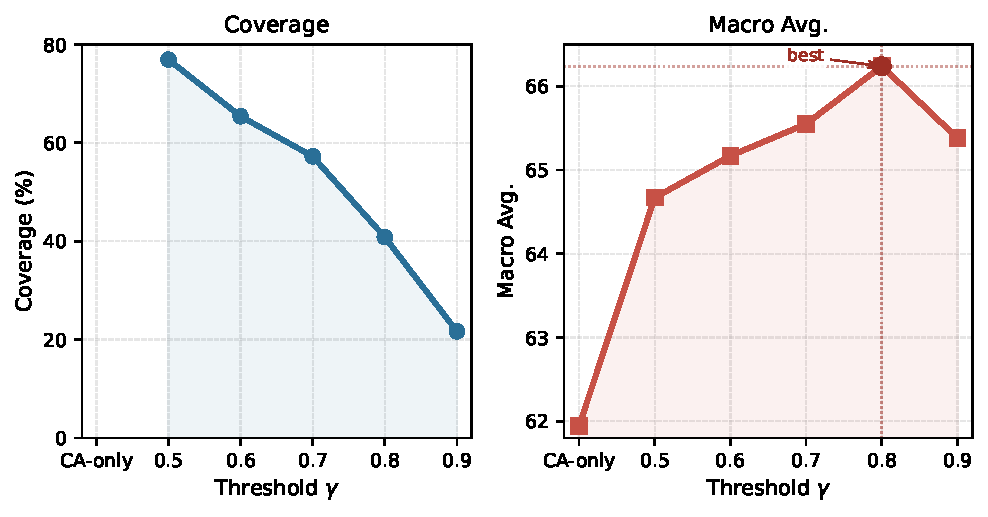
\includegraphics[scale=0.43]{figures/threshold_sensitivity_curve.pdf}
\caption{Threshold sensitivity on Global-MMLU with CA-SFT. Coverage denotes the percentage of test examples that receive memory injection.}
\label{fig:threshold}
\end{figure}

% For each test instance, CA-Mem first generates an English concept and description using CA-only, then retrieves Top-1 memory using subject, generated concept, and generated description. Memory is injected only if the Top-1 similarity score is at least $\gamma$. Figure~\ref{fig:threshold} shows that the best setting remains $\gamma = 0.8$, which trades lower coverage for higher memory precision. Additional Top-k sensitivity, English results, and memory impact analysis are reported in Appendix~\ref{sec:app_additional_results}, while cross-model family generalization is discussed in Section~\ref{sec:cross_model_generalization}.

Figure~\ref{fig:threshold} shows a clear trade-off between memory precision and injection coverage as the retrieval confidence threshold $\gamma$ changes.
A permissive threshold ($\gamma=0.5$) triggers memory augmentation for 76.91\% of the test instances but yields a sub-optimal Macro Average (64.67) due to the incorporation of loosely aligned, noisy heuristics.
Tightening the threshold systematically filters this cross-lingual interference, maximizing reasoning accuracy at 66.24 under $\gamma=0.8$, corresponding to a moderate coverage rate of 40.83\%.
Conversely, an overly high threshold ($\gamma=0.9$) restricts coverage to 21.68\%, discarding valid procedural knowledge and causing a performance regression to 65.38.
This identifies $\gamma=0.8$ as the best equilibrium in our setting, suggesting that high-precision conceptual matching is preferable to broad but noisy memory injection.

\subsection{Cross-Model Family Generalization}
\label{sec:cross_model_generalization}

\begin{figure}[t]
\centering
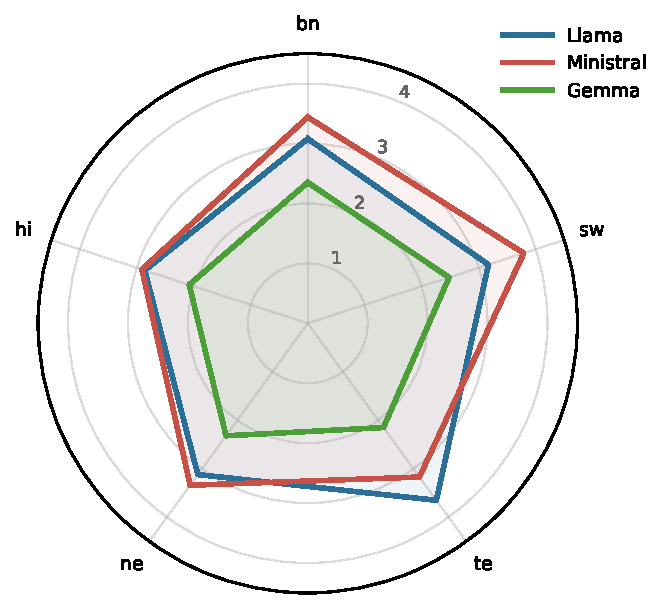
\includegraphics[width=\columnwidth]{figures/cross_model_memory_gain_radar.pdf}
\caption{Per-language memory gains of CA-Mem over CA-only across model families on Global-MMLU.}
\label{fig:cross_model_radar}
\end{figure}

% To examine whether CA-Mem depends on a specific backbone, we evaluate the same memory-augmented inference pipeline on additional model families. Table~\ref{tab:cross_model} in the appendix reports the full results for Llama-3.1-8B-Instruct, Ministral-3-8B-Instruct-2512, and Gemma-3-12B-it. Figure~\ref{fig:cross_model_radar} visualizes the per-language gains of CA-Mem over CA-only. The gains are positive across all evaluated model families and language splits, suggesting that concept-aligned memory provides architecture-robust benefits rather than overfitting to a single base model.

The cross-model evaluation in Figure~\ref{fig:cross_model_radar} suggests that CA-Mem's benefits are not tied to a single backbone.
Applying the memory-augmented pipeline to Llama-3.1-8B-Instruct~\citep{grattafiori2024llama}, Ministral-3-8B-Instruct-2512~\citep{liu2026ministral}, and Gemma-3-12B-it~\citep{gemma2025gemma3} yields consistent positive increments over the memory-free baseline (CA-only).
Specifically, procedural memory injection yields macro-average gains of $+3.18$, $+3.33$, and $+2.27$ across the respective families.
The uniform outward expansion in the radar visualization indicates that these gains are broadly observed across all five evaluated LRLs rather than driven by a single linguistic split.
This pattern indicates that concept-aligned memory leverages generalized semantic representations across model families.

\subsection{Additional Validation}
\vspace{-0.25em}
To ensure that the observed gains are not merely caused by adding extra retrieved context, we conduct setting-matched raw-memory controls in Appendix~\ref{sec:app_additional_validation}. Sanitized raw QA memory, raw trajectory memory, and concept-key raw QA memory all underperform curated procedural memory under the same CA-SFT checkpoint, retrieval encoder, Top-1 retrieval, threshold, fallback behavior, and decoding setting. Appendix~\ref{sec:app_prediction_flip} further shows that CA-Mem rescues substantially more CA-only errors than it introduces new mistakes, while Appendix~\ref{sec:app_inference_cost} shows that CA-Mem adds only modest overhead over CA-only and remains cheaper than SoT.

%%%%%%%%%%%%%%%%%%%%%%%%%%%%%%%%%%%%%%%%%%%%%%%%%%%%%%%%%%%%%%%%%%%%%%%%%%%%%%%%%
\vspace{-0.8em}
\section{Conclusion}
\vspace{-0.55em}

To overcome the cross-lingual knowledge bottleneck in low-resource reasoning, we introduce the Concept-Anchored Memory Agent.
By explicitly abstracting fragile surface inputs into high-resource conceptual definitions, the framework supports more reliable knowledge routing within the pre-trained latent space.
This semantic anchor subsequently retrieves procedural heuristics from a curated Concept Usage Memory, mitigating representation mismatch and reducing redundant contexts in standard retrieval-style pipelines.
Extensive evaluations across diverse multilingual benchmarks and model architectures indicate that injecting concept-aligned experiential knowledge helps reduce reasoning drift.
This methodology offers a scalable direction from passive text conversion to explicit conceptual alignment for multilingual reasoning systems.

\section*{Limitations}

CA-Mem relies on the quality of the initial concept activation step; when the generated concept is overly broad or incorrect, retrieval may return mismatched procedural memory and provide only limited benefit.
Although CA-Mem is designed to support continual memory growth, our evaluation freezes memory snapshots during test-time inference for fair comparison and leakage control; online memory update policies and their stability remain future work.
Our current evaluation focuses on multilingual QA and reasoning benchmarks rather than fully interactive tool-use environments, leaving longer-horizon agent tasks and multimodal settings for future study.


% Bibliography entries for the entire Anthology, followed by custom entries
%\bibliography{anthology,custom}
% Custom bibliography entries only
\bibliography{custom}

\clearpage
\appendix
\section*{Appendix}
\raggedbottom

\section{Dataset and Evaluation Details}
\label{sec:app_dataset}

\begin{table}[H]
\centering
\scriptsize
\setlength{\tabcolsep}{4pt}
\begin{tabular}{l l l r}
\hline
Benchmark & Code & Language & \#Examples \\
\hline
Global-MMLU & bn & Bengali & 14,042 \\
Global-MMLU & sw & Swahili & 14,042 \\
Global-MMLU & te & Telugu & 14,042 \\
Global-MMLU & ne & Nepali & 14,042 \\
Global-MMLU & hi & Hindi & 14,042 \\
Global-MMLU & en & English & 14,042 \\
Global-MMLU & zh & Chinese & 14,042 \\
\hline
INCLUDE & bn & Bengali & 548 \\
INCLUDE & te & Telugu & 548 \\
INCLUDE & ne & Nepali & 500 \\
INCLUDE & hi & Hindi & 547 \\
\hline
MGSM & en & English & 250 \\
MGSM & bn & Bengali & 250 \\
MGSM & sw & Swahili & 250 \\
MGSM & te & Telugu & 250 \\
\hline
\end{tabular}
\caption{Language-level evaluation sizes for the benchmarks discussed in this paper.}
\label{tab:dataset_language_counts}
\end{table}
\FloatBarrier

Global-MMLU \citep{singh2025global} includes Bengali, Swahili, Telugu, Nepali, Hindi, English, and Chinese splits, with 14,042 examples per language.
In the main experiments, we report per-language accuracy and Macro Avg. on the five low-resource languages, while retaining the English and Chinese splits for additional generalization tests.
INCLUDE \citep{romanou2025include} evaluates multilingual examination QA on Bengali, Telugu, Nepali, and Hindi, and we report Weighted Avg. because language-specific test sizes differ.
MGSM \citep{shi2022language} evaluates multilingual math word problem solving on Bengali, Swahili, and Telugu, with 250 examples per language, and we report Macro Avg.

We use benchmark-specific answer extraction and normalization rules consistent with the evaluation setup described in the main text.

\section{Additional Benchmark Results}
\label{sec:app_additional_benchmark_results}

\begin{table*}[t]
\centering
\scriptsize
\setlength{\tabcolsep}{1.5pt}
\renewcommand{\arraystretch}{0.90}
\begin{tabular*}{\textwidth}{@{\extracolsep{\fill}} c l c c c c c c c c c}
\hline
& & \multicolumn{5}{c}{INCLUDE} & \multicolumn{4}{c}{MGSM} \\
\cline{3-7}\cline{8-11}
Model & Method & bn & te & ne & hi & W. Avg. & bn & sw & te & M. Avg. \\
\hline
 & Zero-shot & 49.82 & 37.04 & 48.60 & 57.40 & 48.20 & 17.20 & 16.00 & 8.80 & 14.00 \\
 & CoT & 52.19 & 37.23 & 48.80 & 58.68 & 49.23 & 20.80 & 20.80 & 13.20 & 18.27 \\
 & Cross-CoT & 54.01 & 37.41 & 49.00 & 59.60 & 50.02 & 23.60 & 23.20 & 16.00 & 20.93 \\
Base & Self-Translate & 56.02 & 37.41 & 46.80 & 56.67 & 49.28 & 24.80 & 22.80 & 15.60 & 21.07 \\
 & SoT & 53.83 & 37.41 & 49.20 & 57.59 & 49.51 & 25.20 & 25.60 & 18.00 & 22.93 \\
 & CA-only & 55.47 & 37.59 & 48.80 & 60.69 & 50.67 & 24.80 & 25.60 & 17.60 & 22.67 \\
 & CA-Mem & \textbf{59.85} & \textbf{42.88} & \textbf{53.60} & \textbf{62.89} & \textbf{54.83} & \textbf{27.60} & \textbf{28.00} & \textbf{20.80} & \textbf{25.47} \\
\cline{1-11}
 & Zero-shot & 49.27 & 38.87 & 49.60 & 56.67 & 48.58 & 18.00 & 16.80 & 11.20 & 15.33 \\
 & CoT & 51.64 & 39.23 & 50.40 & 58.32 & 49.88 & 22.00 & 21.20 & 15.60 & 19.60 \\
 & Cross-CoT & 52.55 & 39.42 & 51.00 & 59.05 & 50.49 & 24.00 & 23.60 & 17.20 & 21.60 \\
Direct-SFT & Self-Translate & 54.01 & 40.33 & 52.60 & 59.41 & 51.56 & 25.20 & 23.60 & 16.40 & 21.73 \\
 & SoT & 52.19 & 39.78 & 52.60 & 59.41 & 50.96 & 25.60 & 25.20 & 18.80 & 23.20 \\
 & CA-only & 54.74 & 40.88 & 53.20 & 60.15 & 52.22 & 26.40 & 25.60 & 19.60 & 23.87 \\
 & CA-Mem & \textbf{59.12} & \textbf{44.89} & \textbf{56.40} & \textbf{63.44} & \textbf{55.95} & \textbf{29.20} & \textbf{28.40} & \textbf{22.40} & \textbf{26.67} \\
\cline{1-11}
 & Zero-shot & 51.46 & 39.05 & 51.00 & 59.41 & 50.21 & 20.00 & 17.20 & 12.00 & 16.40 \\
 & CoT & 54.01 & 40.88 & 53.40 & 61.79 & 52.50 & 23.20 & 21.60 & 16.40 & 20.40 \\
 & Cross-CoT & 55.47 & 42.34 & 55.00 & 63.07 & 53.94 & 25.60 & 23.20 & 18.00 & 22.27 \\
CA-SFT & Self-Translate & 56.75 & 41.24 & 52.60 & 62.89 & 53.38 & 25.60 & 24.40 & 16.80 & 22.27 \\
 & SoT & 54.93 & 42.52 & 56.80 & 63.44 & 54.37 & 26.80 & 25.60 & 19.60 & 24.00 \\
 & CA-only & 56.38 & 43.80 & 55.60 & 63.99 & 54.92 & 28.00 & 26.40 & 20.40 & 24.93 \\
 & CA-Mem & \textbf{60.95} & \textbf{47.63} & \textbf{60.40} & \textbf{67.64} & \textbf{59.12} & \textbf{30.80} & \textbf{29.60} & \textbf{23.60} & \textbf{28.00} \\
\hline
\end{tabular*}
\caption{Full INCLUDE and MGSM results in a single merged table. CA-Mem denotes CA-only with concept usage memory.}
\label{tab:include_mgsm_results}
\end{table*}

The gains on MGSM are smaller than those on Global-MMLU and INCLUDE. This pattern is consistent with MGSM consisting of math word problems, where structured decomposition methods such as SoT naturally align with the required multi-step arithmetic reasoning. Nevertheless, CA-Mem still improves over SoT under CA-SFT, indicating that concept-aligned procedural memory remains complementary even when the task format already favors structured reasoning.

\section{Training and Implementation Details}
\label{sec:app_impl}
Table~\ref{tab:implementation_details} summarizes the fine-tuning, retrieval, and decoding settings used in the experiments.

\begin{table}[!htbp]
\centering
\scriptsize
\setlength{\tabcolsep}{6pt}
\begin{tabular}{l l}
\hline
Item & Value \\
\hline
Base model & Qwen3.5-9B~\citep{qwen35} \\
Fine-tuning & 4-bit QLoRA~\citep{dettmers2023qlora} \\
LoRA rank & 64 \\
LoRA alpha & 128 \\
LoRA dropout & 0.05 \\
Max sequence length & 2048 \\
Batch size & 2 per GPU \\
Gradient accumulation & 16 \\
Learning rate & 2e-4 \\
Epochs & 2 \\
Scheduler & cosine \\
Retrieval encoder & BAAI/bge-m3~\citep{chen2024bge} \\
Decoding temperature & 0 \\
\hline
\end{tabular}
\caption{Implementation details used in the current setup.}
\label{tab:implementation_details}
\end{table}
\FloatBarrier

\paragraph{Artifact use and licenses.}
We use publicly available benchmarks and model artifacts only for research evaluation and method development, following their released licenses or usage terms. The used artifacts include Global-MMLU, INCLUDE, MGSM, MMLU-ProX, Qwen3.5-9B, BGE-M3, Llama, Ministral, and Gemma. We do not redistribute benchmark test sets, evaluation answers, or proprietary model outputs. The constructed memory entries are answer-sanitized and exclude source questions, options, answer labels, gold answers, correct options, and answer-bearing shortcuts.

\section{Prompt Templates}
\label{sec:app_prompts}
\subsection{Prompt Templates for Concept Distillation, CA-SFT, and Evaluation}

The prompt templates below are written in the Global-MMLU format, where each input consists of a question and labeled answer options. INCLUDE is also a multiple-choice benchmark and uses the same prompt format. MGSM is instantiated with the same method-specific prompts but without answer options; its final \texttt{answer} field is the normalized final answer rather than an option label.

For methods that construct an intermediate representation, we use a two-stage evaluation protocol. The first stage generates the method-specific intermediate representation without producing the final answer. The second stage predicts the answer from the intermediate representation and the benchmark input fields required by that method. For Cross-CoT, SoT, CA-only, and CA-Mem, the original question and options are retained in the second stage; for Self-Translate, the second stage uses the translated English question and options. For CA-Mem, memory retrieval is performed between the two stages: after concept activation, we construct the retrieval query by concatenating the subject, activated concept, and concept description. The retrieved usage summary is then provided to the second-stage answer prompt. The retrieved memory is not generated by the LLM.

All methods are evaluated only by the final \texttt{answer} field.

\subsection{Concept Distillation and CA-SFT Prompts}

\begin{promptbox}{Teacher Prompt for Concept Distillation}
\textbf{Task:} \texttt{concept\_distillation}\\
\textbf{Language:} \texttt{<language>}\\
\textbf{Subject:} \texttt{<subject>}

You are given a multilingual multiple-choice question with answer options.
\end{promptbox}

\begin{promptcontbox}
\textbf{Task.} Produce a high-quality supervision tuple for concept-anchored reasoning.

\textbf{You must output three fields.} \texttt{concept}: a concise English concept cue that captures the key knowledge, rule, or reasoning skill required by the question. \texttt{description}: a short English definition of the concept that explains it generally and is reusable for similar questions. \texttt{answer}: the correct option label.

\textbf{Requirements for concept.} Must be written in English; concise and informative; domain-appropriate for the subject; centered on the key knowledge or reasoning operation; not a generic label such as ``reasoning'' or ``multiple-choice''; not contain the answer label; not directly reveal the correct option; reusable beyond this question.

\textbf{Requirements for description.} Must be written in English; define the general concept, rule, or reasoning skill; describe when or how the concept is used; not provide a step-by-step solution to the current question; not mention the correct option; not copy long spans from the question or options; avoid overly broad or vague wording.

\textbf{Requirements for answer.} Must be exactly one option label from the provided options.

\textbf{Self-check before returning.} Verify that the answer is consistent with the question and options, the concept is necessary for solving the question, and the description is reusable and free of answer leakage.
\end{promptcontbox}

\begin{promptcontbox}
Return a valid JSON object only:
{\ttfamily\scriptsize
\noindent \{\\
\quad "concept": "...",\\
\quad "description": "...",\\
\quad "answer": "..."\\
\}
\par
}

\textbf{Question:} \texttt{<question>}\\
\textbf{Options:} \texttt{<options>}
\end{promptcontbox}

\begin{promptbox}{CA-SFT Prompt for Concept Generation}
\textbf{Task:} \texttt{generate\_concept}\\
\textbf{Language:} \texttt{<language>}\\
\textbf{Subject:} \texttt{<subject>}

You are given a multilingual multiple-choice question.
\end{promptbox}

\begin{promptcontbox}
\textbf{Task.} Extract a reusable English concept cue and a short English concept description.

\textbf{Requirements for concept.} Must be written in English; concise and informative; domain-appropriate for the subject; capture the key knowledge, rule, or reasoning skill required by the question; not be a generic label such as ``reasoning,'' ``knowledge,'' or ``multiple-choice''; not contain the answer label; not directly reveal the correct option.

\textbf{Requirements for description.} Must be written in English; define or explain the concept in general terms; be reusable for similar questions; not solve the current question step by step; not mention the correct option; not copy long spans from the question or options.
\end{promptcontbox}

\begin{promptcontbox}
Return a valid JSON object only:
{\ttfamily\scriptsize
\noindent \{\\
\quad "concept": "...",\\
\quad "description": "..."\\
\}
\par
}

\textbf{Question:} \texttt{<question>}\\
\textbf{Options:} \texttt{<options>}
\end{promptcontbox}

\begin{promptbox}{CA-SFT Prompt for Concept-Grounded Answering}
\textbf{Task:} \texttt{answer\_with\_concept}\\
\textbf{Language:} \texttt{<language>}\\
\textbf{Subject:} \texttt{<subject>}

You are given: 1. a multilingual multiple-choice question; 2. an activated English concept; 3. a short English description of the concept.
\end{promptbox}

\begin{promptcontbox}
\textbf{Task.} Use the concept and description as auxiliary guidance to select the single best answer.

\textbf{Rules.} The question and options are authoritative. The concept and description are auxiliary cues, not replacements for the question. If the concept or description is partially mismatched, rely on the question and options. Do not force the question to fit the concept. Do not invent missing facts. Do not provide explanation. The final answer must be one of the option labels exactly as given.
\end{promptcontbox}

\begin{promptcontbox}
Return a valid JSON object only:
{\ttfamily\scriptsize
\noindent \{\\
\quad "answer": "..."\\
\}
\par
}

\textbf{Activated concept:} \texttt{<concept>}\\
\textbf{Concept description:} \texttt{<description>}\\
\textbf{Question:} \texttt{<question>}\\
\textbf{Options:} \texttt{<options>}
\end{promptcontbox}

\begin{promptbox}{LLM Judge Prompt for Concept Filtering}
\textbf{Task:} \texttt{concept\_quality\_judgment}

You are evaluating whether a distilled concept-description pair is useful for solving a multilingual multiple-choice question.
\end{promptbox}

\begin{promptcontbox}
\textbf{Input.} \texttt{Language: <language>} \texttt{Subject: <subject>} \texttt{Question: <question>} \texttt{Options: <options>} \texttt{Gold answer: <gold\_answer>} \texttt{Teacher answer: <teacher\_answer>} \texttt{Distilled concept: <concept>} \texttt{Distilled description: <description>}

\textbf{Scoring scale.} For \texttt{relevance}, \texttt{specificity}, \texttt{description\_quality}, and \texttt{reusability}: 1 = poor, 2 = weak, 3 = acceptable, 4 = good, 5 = excellent. For \texttt{risk}: 1 = very low risk, 2 = low risk, 3 = moderate risk, 4 = high risk, 5 = very high risk. The risk direction is reversed: higher risk is worse.

\textbf{Criteria.} \texttt{relevance}: whether the concept captures the knowledge, rule, or reasoning skill needed to answer the question. \texttt{specificity}: whether the concept is informative rather than overly generic. \texttt{description\_quality}: whether the description correctly and clearly defines the concept in general terms. \texttt{reusability}: whether the concept and description can be reused beyond this exact instance. \texttt{risk}: whether the concept or description is misleading, answer-specific, shortcut-inducing, overfit to the current question, mismatched, or likely to harm downstream reasoning.

\textbf{Important.} Do not reward a concept merely because the teacher answer is correct. Penalize answer leakage, option-specific shortcuts, vague concepts such as ``basic knowledge,'' and descriptions that solve the instance step by step instead of defining reusable knowledge.
\end{promptcontbox}

\begin{promptcontbox}
Return a valid JSON object only:
{\ttfamily\scriptsize
\noindent \{\\
\quad "relevance": ...,\\
\quad "specificity": ...,\\
\quad "description\_quality": ...,\\
\quad "reusability": ...,\\
\quad "risk": ...,\\
\quad "rationale": "..."\\
\}
\par
}
\end{promptcontbox}


\subsection{Memory Curation Prompt}

\begin{promptbox}{Memory Curator Prompt for Concept Usage Memory}
\textbf{Task:} \texttt{memory\_curation}\\
\textbf{Language:} \texttt{<language>}\\
\textbf{Subject:} \texttt{<subject>}

You are given a source-side solving trajectory produced by a teacher model and evaluated by an external verifier.
Your task is to curate an answer-sanitized concept usage memory node from the solving trajectory and verifier feedback.

The memory node should capture reusable procedural knowledge about how to apply the activated concept.
It must not preserve the original question, option text, answer label, gold answer, or any answer-bearing shortcut.
\end{promptbox}

\begin{promptcontbox}
\textbf{Task.}
Construct a reusable memory node with the following fields: \texttt{subject}, \texttt{concept}, \texttt{description}, and \texttt{usage\_summary}.

The \texttt{usage\_summary} must be organized into three procedural components: \texttt{trigger\_invariants}, \texttt{decision\_rules}, and \texttt{negative\_error\_boundaries}.

\textbf{Definitions.}
\texttt{trigger\_invariants} describe when the concept should be activated, including stable cues, conditions, or problem patterns that indicate the concept is relevant.

\texttt{decision\_rules} describe how to apply the concept once it is activated, including reusable reasoning operations, comparisons, constraints, or calculation principles.

\texttt{negative\_error\_boundaries} describe what should not be assumed or what mistakes should be avoided, including common confusions, invalid shortcuts, distractor patterns, or boundary cases.
\end{promptcontbox}

\begin{promptcontbox}
\textbf{Requirements.}
The memory node must be written in English.
It must describe reusable procedural guidance rather than a solution to the current instance.
It must be reusable for future questions in the same subject area.
It must not copy the source question.
It must not copy any option text.
It must not mention the model's final answer label.
It must not mention the gold answer.
It must not reveal the correct option.
It must not include answer-bearing shortcuts.
It must not store a worked solution to the source question.
It must avoid source-specific entities, numbers, or surface details unless they are necessary to define the general concept.

\textbf{Quality control.}
Set \texttt{keep} to \texttt{true} only if the trajectory is verifier-approved and the memory node is general, reusable, answer-sanitized, and aligned with the activated concept.
Set \texttt{keep} to \texttt{false} if the trajectory is not verifier-approved, the concept is too vague, the usage summary leaks the answer, copies the instance, or cannot be reused.
\end{promptcontbox}

\begin{promptcontbox}
Return a valid JSON object only:
{\ttfamily\scriptsize
\noindent \{\\
\quad "keep": true,\\
\quad "subject": "...",\\
\quad "concept": "...",\\
\quad "description": "...",\\
\quad "usage\_summary": \{\\
\quad\quad "trigger\_invariants": "...",\\
\quad\quad "decision\_rules": "...",\\
\quad\quad "negative\_error\_boundaries": "..."\\
\quad \},\\
\quad "drop\_reason": ""\\
\}
\par
}
\end{promptcontbox}

\begin{promptcontbox}
If the memory node should be discarded, return:
{\ttfamily\scriptsize
\noindent \{\\
\quad "keep": false,\\
\quad "subject": "...",\\
\quad "concept": "...",\\
\quad "description": "...",\\
\quad "usage\_summary": \{\\
\quad\quad "trigger\_invariants": "",\\
\quad\quad "decision\_rules": "",\\
\quad\quad "negative\_error\_boundaries": ""\\
\quad \},\\
\quad "drop\_reason": "..."\\
\}
\par
}
\end{promptcontbox}

\begin{promptcontbox}
\textbf{Question:} \texttt{<question>}\\
\textbf{Options:} \texttt{<options>}\\
\textbf{Activated concept:} \texttt{<concept>}\\
\textbf{Concept description:} \texttt{<description>}\\
\textbf{Teacher solving trajectory:} \texttt{<solution\_trace>}\\
\textbf{Teacher prediction:} \texttt{<teacher\_prediction>}\\
\textbf{Verification status:} \texttt{<verification\_status>}\\
\textbf{Verifier feedback:} \texttt{<verifier\_feedback>}
\end{promptcontbox}

\subsection{Evaluation-Time Prompt Templates}

\begin{promptbox}{Zero-Shot Evaluation Prompt}
\textbf{Method:} Zero-shot\\
\textbf{Language:} \texttt{<language>}\\
\textbf{Subject:} \texttt{<subject>}

You are given a multiple-choice question in \texttt{<language>}.
\end{promptbox}

\begin{promptcontbox}
\textbf{Task.} Select the single best answer from the provided options.

\textbf{Rules.} Read the question and all options carefully. Do not provide explanation. Do not invent information not supported by the question or options. The answer must be one of the option labels exactly as given. Preserve the original option label format.

Return a valid JSON object only:
{\ttfamily\scriptsize
\noindent \{\\
\quad "answer": "..."\\
\}
\par
}

\textbf{Question:} \texttt{<question>}\\
\textbf{Options:} \texttt{<options>}
\end{promptcontbox}

\begin{promptbox}{CoT Evaluation Prompt}
\textbf{Method:} Chain-of-Thought\\
\textbf{Language:} \texttt{<language>}\\
\textbf{Subject:} \texttt{<subject>}

You are given a multiple-choice question in \texttt{<language>}.
\end{promptbox}

\begin{promptcontbox}
\textbf{Task.} Reason step by step, then select the single best answer.

\textbf{Rules.} Reason in English when possible. Preserve all quantities, entities, units, negations, and option labels. Do not ignore any condition in the question. Do not invent information not supported by the question or options. The final answer must be one of the option labels exactly as given.

Return a valid JSON object only:
{\ttfamily\scriptsize
\noindent \{\\
\quad "reasoning": "...",\\
\quad "answer": "..."\\
\}
\par
}

\textbf{Question:} \texttt{<question>}\\
\textbf{Options:} \texttt{<options>}
\end{promptcontbox}

\subsection{Two-Stage Baseline Prompts}

\begin{promptbox}{Cross-CoT Stage 1}
\textbf{Method:} Cross-CoT, Stage 1\\
\textbf{Language:} \texttt{<language>}\\
\textbf{Subject:} \texttt{<subject>}

You are given a multilingual multiple-choice question.
\end{promptbox}

\begin{promptcontbox}
\textbf{Task.} Understand the question in its original language and produce a high-resource-language reasoning trace in English.

\textbf{Rules.} Reason in English. Preserve all numbers, units, named entities, negations, comparisons, and option labels. Do not mechanically translate the entire question word by word. Focus on the knowledge, constraints, and reasoning steps needed to solve the question. Do not output the final answer label. Do not state ``the answer is \ldots'' Do not invent information not supported by the question or options.

Return a valid JSON object only:
{\ttfamily\scriptsize
\noindent \{\\
\quad "english\_reasoning": "..."\\
\}
\par
}

\textbf{Question:} \texttt{<question>}\\
\textbf{Options:} \texttt{<options>}
\end{promptcontbox}

\begin{promptbox}{Cross-CoT Stage 2}
\textbf{Method:} Cross-CoT, Stage 2\\
\textbf{Language:} \texttt{<language>}\\
\textbf{Subject:} \texttt{<subject>}

You are given: 1. the original multilingual multiple-choice question; 2. the original answer options; 3. an English reasoning trace produced from the question.
\end{promptbox}

\begin{promptcontbox}
\textbf{Task.} Select the single best answer using the question, options, and English reasoning trace.

\textbf{Rules.} The original question and options are authoritative. Use the English reasoning trace as auxiliary guidance. If the reasoning trace appears partially incorrect, incomplete, or mismatched, rely on the original question and options. Do not provide explanation. The final answer must be one of the option labels exactly as given. Preserve the original option label format.

Return a valid JSON object only:
{\ttfamily\scriptsize
\noindent \{\\
\quad "answer": "..."\\
\}
\par
}

\textbf{English reasoning:} \texttt{<english\_reasoning>}\\
\textbf{Question:} \texttt{<question>}\\
\textbf{Options:} \texttt{<options>}
\end{promptcontbox}

\begin{promptbox}{Self-Translate Stage 1}
\textbf{Method:} Self-Translate, Stage 1\\
\textbf{Language:} \texttt{<language>}

Translate or faithfully rephrase the following multiple-choice question into English.
\end{promptbox}

\begin{promptcontbox}
\textbf{Rules.} Do not answer the question. Do not explain. Preserve all numbers, units, formulas, named entities, negations, and option labels. Keep the original option structure. Translate the question and options faithfully. If a term should not be translated, preserve it.

Return a valid JSON object only:
{\ttfamily\scriptsize
\noindent \{\\
\quad "english\_question": "...",\\
\quad "english\_options": "..."\\
\}
\par
}

\textbf{Question:} \texttt{<question>}\\
\textbf{Options:} \texttt{<options>}
\end{promptcontbox}

\begin{promptbox}{Self-Translate Stage 2}
\textbf{Method:} Self-Translate, Stage 2\\
\textbf{Language:} English\\
\textbf{Subject:} \texttt{<subject>}

You are given an English translation or rephrasing of a multilingual multiple-choice question.
\end{promptbox}

\begin{promptcontbox}
\textbf{Task.} Select the single best answer from the translated English question and options.

\textbf{Rules.} Use only the translated question and options. Preserve the original option labels exactly. Do not provide explanation. Do not invent information not supported by the question or options. The final answer must be one of the option labels exactly as given.

Return a valid JSON object only:
{\ttfamily\scriptsize
\noindent \{\\
\quad "answer": "..."\\
\}
\par
}

\textbf{Translated question:} \texttt{<english\_question>}\\
\textbf{Translated options:} \texttt{<english\_options>}
\end{promptcontbox}

\begin{promptbox}{SoT Stage 1}
\textbf{Method:} SoT, Stage 1\\
\textbf{Language:} \texttt{<language>}\\
\textbf{Subject:} \texttt{<subject>}

You are given a multilingual multiple-choice question.
\end{promptbox}

\begin{promptcontbox}
\textbf{Task.} Convert the problem into a compact structured representation for reasoning.

\textbf{Steps.} Identify the essential meaning of the question. Extract key entities, quantities, units, conditions, relations, and the target variable. Preserve negations, comparisons, constraints, and option labels. Represent the problem in a language-agnostic structured form.

\textbf{Rules.} Do not output the final answer label. Do not state ``the answer is \ldots'' Do not solve the question step by step. Do not invent facts not present in the question or options. The structure should be concise but sufficient for answering. Preserve the original option labels exactly.
\end{promptcontbox}

\begin{promptcontbox}
Return a valid JSON object only:
{\ttfamily\scriptsize
\noindent \{\\
\quad "structure": \{\\
\quad\quad "question\_intent": "...",\\
\quad\quad "entities": ["..."],\\
\quad\quad "conditions": ["..."],\\
\quad\quad "relations": ["..."],\\
\quad\quad "target": "...",\\
\quad\quad "option\_map": \{"<label>": "..."\}\\
\quad \}\\
\}
\par
}

\textbf{Question:} \texttt{<question>}\\
\textbf{Options:} \texttt{<options>}
\end{promptcontbox}

\begin{promptbox}{SoT Stage 2}
\textbf{Method:} SoT, Stage 2\\
\textbf{Language:} \texttt{<language>}\\
\textbf{Subject:} \texttt{<subject>}

You are given: 1. the original multilingual multiple-choice question; 2. the original answer options; 3. a structured representation of the problem.
\end{promptbox}

\begin{promptcontbox}
\textbf{Task.} Select the single best answer using the structured representation.

\textbf{Rules.} The original question and options are authoritative. Use the structure as auxiliary guidance. If the structure is incomplete, incorrect, or partially mismatched, rely on the original question and options. Check all constraints, negations, quantities, units, and option labels before answering. Do not provide explanation. The final answer must be one of the option labels exactly as given.

Return a valid JSON object only:
{\ttfamily\scriptsize
\noindent \{\\
\quad "answer": "..."\\
\}
\par
}

\textbf{Structured representation:} \texttt{<structure>}\\
\textbf{Question:} \texttt{<question>}\\
\textbf{Options:} \texttt{<options>}
\end{promptcontbox}

\subsection{CA-Mem Evaluation Prompts}

\begin{promptbox}{CA-only / CA-Mem Stage 1: Concept Activation}
\textbf{Method:} CA-only / CA-Mem, Stage 1\\
\textbf{Language:} \texttt{<language>}\\
\textbf{Subject:} \texttt{<subject>}

You are given a multilingual multiple-choice question.
\end{promptbox}

\begin{promptcontbox}
\textbf{Task.} Activate the core English concept needed to solve the question. The goal is not to translate the full question. The goal is to identify the high-level concept, rule, or reasoning skill required by the question.

\textbf{Requirements for concept.} Must be written in English; concise and informative; domain-appropriate for the given subject; capture the central knowledge or reasoning operation needed by the question; not be a generic label such as ``reasoning,'' ``knowledge,'' or ``multiple-choice''; not contain the answer label; not directly reveal the correct option.

\textbf{Requirements for description.} Must be written in English; define the concept in general terms; describe when or how the concept is used; not solve the specific question step by step; not mention the correct option; not copy long spans from the question or options.

Return a valid JSON object only:
{\ttfamily\scriptsize
\noindent \{\\
\quad "concept": "...",\\
\quad "description": "..."\\
\}
\par
}

\textbf{Question:} \texttt{<question>}\\
\textbf{Options:} \texttt{<options>}
\end{promptcontbox}

\begin{promptbox}{CA-only Stage 2: Concept-Grounded Answering}
\textbf{Method:} CA-only, Stage 2\\
\textbf{Language:} \texttt{<language>}\\
\textbf{Subject:} \texttt{<subject>}

You are given: 1. a multilingual multiple-choice question; 2. an activated English concept; 3. a short English description of the concept.
\end{promptbox}

\begin{promptcontbox}
\textbf{Task.} Use the concept and description as auxiliary guidance to select the single best answer.

\textbf{Rules.} The question and options are authoritative. The concept and description are auxiliary cues, not replacements for the question. If the concept or description is partially mismatched, rely on the question and options. Do not force the question to fit the concept. Do not invent missing facts. Do not provide explanation. The final answer must be one of the option labels exactly as given.

Return a valid JSON object only:
{\ttfamily\scriptsize
\noindent \{\\
\quad "answer": "..."\\
\}
\par
}

\textbf{Activated concept:} \texttt{<concept>}\\
\textbf{Concept description:} \texttt{<description>}\\
\textbf{Question:} \texttt{<question>}\\
\textbf{Options:} \texttt{<options>}
\end{promptcontbox}

\begin{promptbox}{CA-Mem Retrieval Step}
After Stage 1, the retrieved memory is not generated by the LLM. We construct the retrieval query by concatenating the subject, activated concept, and concept description:

{\ttfamily\scriptsize
\noindent retrieval\_query = concat(subject, concept, description)
\par
}

The query is encoded with the retrieval encoder and matched against the frozen concept usage memory bank. We retrieve the Top-1 memory node only when its similarity score is at least $\gamma$. If no memory node passes the threshold, CA-Mem falls back to CA-only.
\end{promptbox}

\begin{promptbox}{CA-Mem Stage 2: Memory-Augmented Answering}
\textbf{Method:} CA-Mem, Stage 2\\
\textbf{Language:} \texttt{<language>}\\
\textbf{Subject:} \texttt{<subject>}

You are given: 1. a multilingual multiple-choice question; 2. an activated English concept and description; 3. a retrieved concept usage memory.

The retrieved memory is obtained from the frozen concept usage memory bank using the subject, activated concept, and concept description as the retrieval query. It contains procedural guidance about how the concept is usually applied and may include trigger conditions, decision rules, and common pitfalls.
\end{promptbox}

\begin{promptcontbox}
\textbf{Task.} Use the concept, description, and retrieved memory as auxiliary guidance to select the single best answer.

\textbf{Rules.} The question and options are authoritative. The concept and description are auxiliary cues, not replacements for the question. Use the retrieved memory only if it is relevant to the activated concept and the current question. If the memory is partially mismatched, ignore the mismatched part. Do not copy an answer from memory. Do not assume that the memory contains the answer to this question. Use the memory to guide concept application, not to replace the question. Check whether any option violates the concept boundary or a known pitfall. Do not provide explanation. The final answer must be one of the option labels exactly as given.
\end{promptcontbox}

\begin{promptcontbox}
Return a valid JSON object only:
{\ttfamily\scriptsize
\noindent \{\\
\quad "answer": "..."\\
\}
\par
}

\textbf{Activated concept:} \texttt{<concept>}\\
\textbf{Concept description:} \texttt{<description>}\\
\textbf{Retrieved usage memory:} \texttt{<usage\_summary>}\\
\textbf{Question:} \texttt{<question>}\\
\textbf{Options:} \texttt{<options>}
\end{promptcontbox}

\subsection{MGSM Adapter}

\begin{promptbox}{MGSM Adapter}
For MGSM, we instantiate the same method-specific prompts without the \texttt{Options} field, since MGSM is evaluated as open-ended math question answering. The final \texttt{answer} field contains the normalized final answer rather than an option label. Intermediate representations, such as English reasoning traces, structured representations, concept-description pairs, and retrieved memory summaries, follow the same method-specific templates.
\end{promptbox}
\subsection{Raw-Memory Baseline Prompts}

\begin{promptbox}{Raw-Memory Baseline Stage 2}
\textbf{Method:} Raw-memory baseline\\
\textbf{Language:} \texttt{<language>}\\
\textbf{Subject:} \texttt{<subject>}

You are given: 1. a multilingual multiple-choice question; 2. a retrieved raw memory snippet.
\end{promptbox}

\begin{promptcontbox}
The retrieved memory snippet may come from sanitized raw QA memory, sanitized raw trajectory memory, or raw QA memory indexed by a concept key. Use it as auxiliary guidance only if it is relevant to the question. The question and options are authoritative. Do not copy an answer from memory. Do not assume the memory contains the correct option. Do not provide explanation. The final answer must be one of the option labels exactly as given.

Return a valid JSON object only:
{\ttfamily\scriptsize
\noindent \{\\
\quad "answer": "..."\\
\}
\par
}

\textbf{Retrieved content:} \texttt{<retrieved\_content>}\\
\textbf{Question:} \texttt{<question>}\\
\textbf{Options:} \texttt{<options>}
\end{promptcontbox}

\subsection{Answer Extraction}

\begin{promptbox}{Final Answer Extraction}
Given a model response, extract the final benchmark answer in the required normalized format. Preserve the option label exactly for multiple-choice tasks and the normalized final answer for MGSM. Do not add explanation.
\end{promptbox}
\FloatBarrier

\section{Leakage Prevention and Memory Construction}
\label{sec:app_leakage_memory}
\subsection{Leakage Prevention}
Before constructing either SFT data or memory nodes, we apply instance-level decontamination between the MMLU-ProX~\citep{xuan2025mmlu} source pool and all evaluation benchmarks, including Global-MMLU, INCLUDE, and MGSM. We remove exact duplicates, normalized duplicates, and answer-equivalent source--test reformulations before both CA-SFT construction and memory curation. We canonicalize each question with Unicode normalization, whitespace normalization, punctuation normalization, lowercasing where applicable, and removal of option-label artifacts. This filtering is instance-level rather than concept-level: we do not remove source examples merely because they share high-level concepts or reasoning skills with evaluation examples, since concept-level transfer is the intended setting. The final memory bank is frozen before evaluation, and test examples only perform read-only retrieval. Memory nodes are answer-sanitized and exclude source questions, option text, answer labels, gold answers, correct-option text, and answer-bearing shortcuts.

\subsection{SFT Data Construction}
For supervised training, we start from the duplicate-filtered MMLU-ProX~\citep{xuan2025mmlu} source pool and apply teacher-correctness filtering followed by an LLM-based concept-quality filter. We retain 4,700 rows for each of the five training languages. Each retained row is converted into two CA-SFT instances: concept generation and concept-grounded answering. Direct-SFT uses the same retained rows but keeps only answer supervision. The filtering criteria for the retained CA-SFT rows are shown in Table~\ref{tab:main_keep_filter}.

\begin{table}[!htbp]
\centering
\scriptsize
\setlength{\tabcolsep}{4pt}
\begin{tabular}{l l}
\hline
Filter & Criterion \\
\hline
Teacher correctness & teacher\_answer == gold \\
Parsing validity & valid concept, description, and answer \\
Risk control & risk $\leq 3$ \\
Overall quality & mean\_score $\geq 3.25$ \\
Relevance & relevance $\geq 3$ \\
Description quality & description\_quality $\geq 3$ \\
\hline
\end{tabular}
\caption{Filtering criteria for the \texttt{main\_keep} split used for concept distillation and CA-SFT construction.}
\label{tab:main_keep_filter}
\end{table}

\noindent The \texttt{main\_keep} criteria above are used for concept distillation and CA-SFT construction. Memory construction uses the same duplicate-filtered source pool but retains only verifier-approved teacher trajectories before curator abstraction.

\noindent\texttt{mean\_score} is computed as the average of relevance, specificity, description\_quality, and reusability. The risk score is not included in \texttt{mean\_score} and is used only as a filtering constraint. The borderline bucket is retained only as a fallback pool; the final 4,700-per-language setting uses the \texttt{main\_keep} split exclusively.

\begin{figure}[!htbp]
\centering
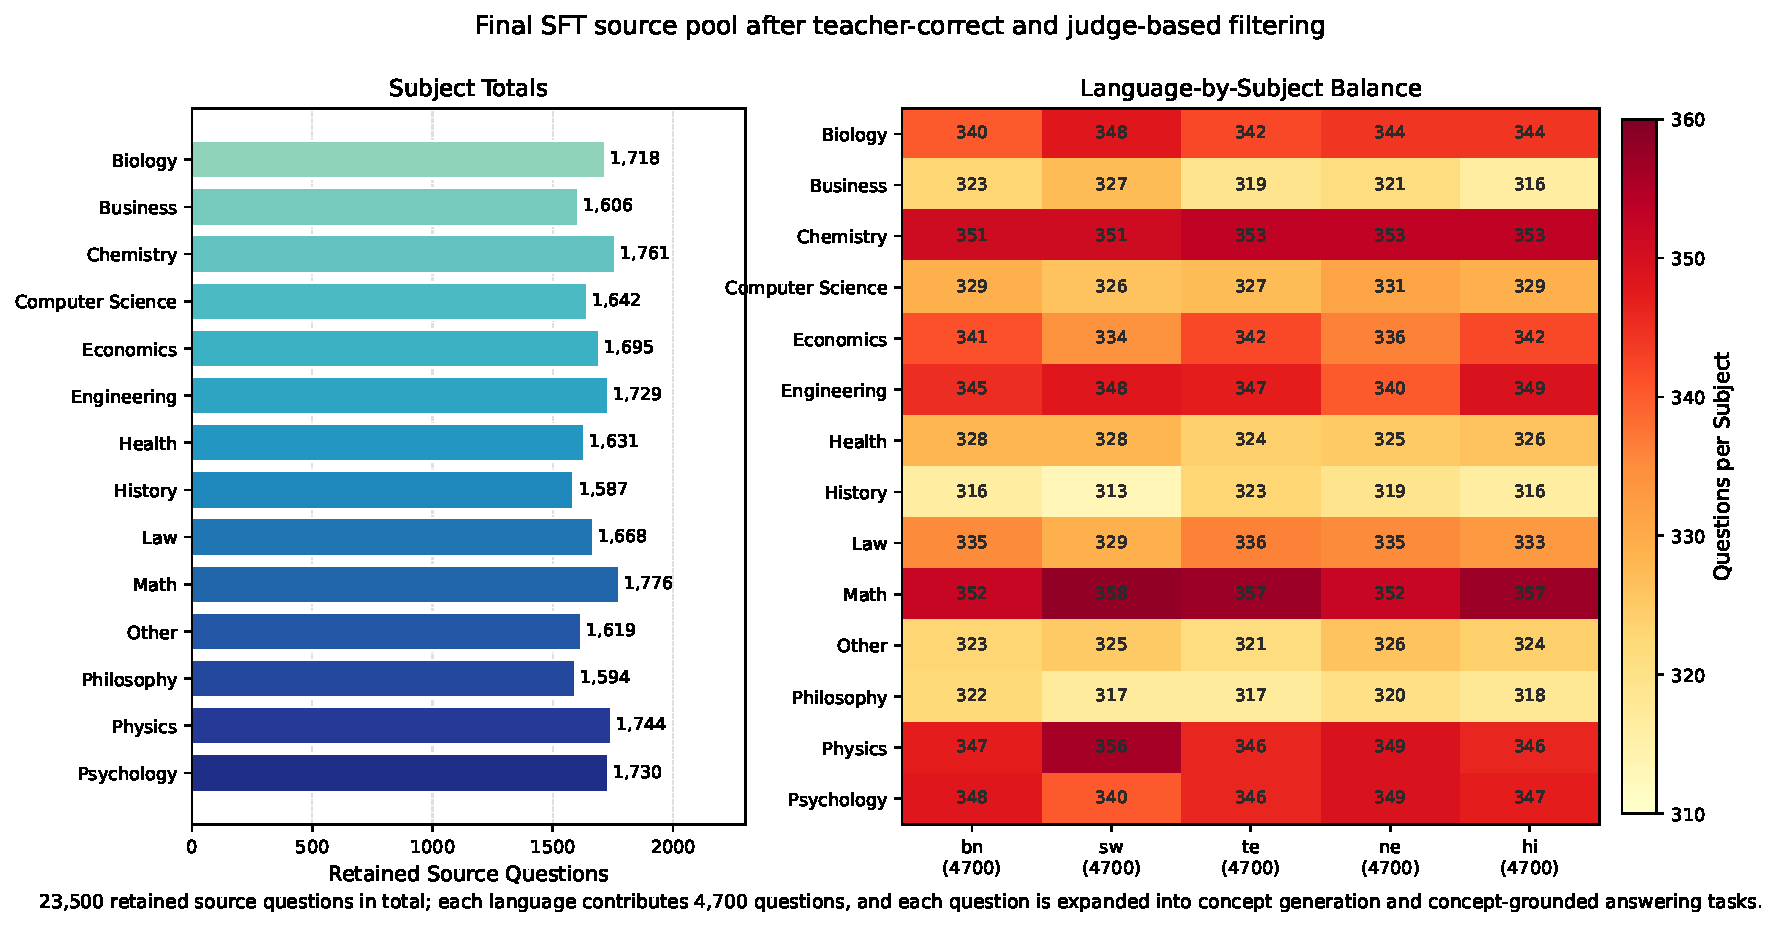
\includegraphics[width=\columnwidth]{figures/sft_subject_distribution.pdf}
\caption{Subject distribution of the final \texttt{main\_keep} source pool used to build the SFT data. The teacher first produces \{concept, description, answer\} in a single response, we keep only teacher-correct samples, and then apply judge-based quality filtering. The final retained CA-SFT pool is evenly balanced across the five training languages, with 4,700 rows per language. Each retained row is later expanded into two CA-SFT instances: concept generation and concept-grounded answering.}
\label{fig:sft_subject_distribution}
\end{figure}
\FloatBarrier

\subsection{Memory Construction}
Memory construction uses the same duplicate-filtered source pool but follows a separate trajectory-based curation pipeline. A teacher model first solves filtered source-side questions and produces solving trajectories. In our implementation, GPT-5.4 is used as the teacher model. An external verifier uses the source-side gold label only to determine whether a trajectory is eligible for curation. Only verifier-approved teacher trajectories are passed to the memory curator. The source-side gold label is not provided as an input field to the memory curator and is not stored in the memory node. From the verified trajectory pool, we construct 6,934 candidate memory nodes and retain 5,087 final concept memory nodes after curation. Each retained node stores an answer-sanitized usage summary with three components: trigger invariants, decision rules, and negative error boundaries. The final memory bank is frozen during evaluation and excludes original source questions, evaluation questions, option text, answer labels, gold answers, correct option text, and answer-bearing shortcuts.
The memory curator prompt, provided in Appendix~\ref{sec:app_prompts}, converts verifier-approved teacher trajectories into answer-sanitized usage summaries with three fields: trigger invariants, decision rules, and negative error boundaries.

\section{Memory Bank Statistics}
\label{sec:app_memory_stats}
This section summarizes the frozen memory bank used in the final experiments.
Table~\ref{tab:memory_bank_stats} reports the overall memory-bank size, Table~\ref{tab:memory_category_distribution} gives the category distribution, and Table~\ref{tab:memory_growth_by_category} shows how category counts grow as more source data is processed.

\begin{table}[!htbp]
\centering
\scriptsize
\setlength{\tabcolsep}{5pt}
\begin{tabular}{l l}
\hline
Statistic & Value \\
\hline
Candidate memory nodes & 6,934 \\
Final concept memory nodes & 5,087 \\
Coarse categories & 14 \\
\hline
\end{tabular}
\caption{Memory bank statistics.}
\label{tab:memory_bank_stats}
\end{table}

\begin{table}[!htbp]
\centering
\scriptsize
\setlength{\tabcolsep}{3pt}
\resizebox{\columnwidth}{!}{%
\begin{tabular}{l r r l r r}
\hline
Category & Nodes & Ratio & Category & Nodes & Ratio \\
\hline
Math & 473 & 9.30\% & Law & 366 & 7.19\% \\
Physics & 428 & 8.41\% & Economics & 342 & 6.72\% \\
Chemistry & 417 & 8.20\% & Psychology & 329 & 6.47\% \\
Biology & 406 & 7.98\% & Business & 317 & 6.23\% \\
Health & 394 & 7.75\% & History & 304 & 5.98\% \\
Computer Science & 383 & 7.53\% & Philosophy & 281 & 5.52\% \\
Engineering & 357 & 7.02\% & Other & 290 & 5.70\% \\
Total & 5,087 & 100\% & & & \\
\hline
\end{tabular}
}
\caption{Category distribution of the final memory bank.}
\label{tab:memory_category_distribution}
\end{table}

\begin{table}[!htbp]
\centering
\scriptsize
\setlength{\tabcolsep}{3pt}
\renewcommand{\arraystretch}{0.96}
\begin{tabular}{l r r r r}
\hline
Category & 25\% & 50\% & 75\% & 100\% \\
\hline
Math & 118 & 237 & 355 & 473 \\
Physics & 107 & 214 & 321 & 428 \\
Chemistry & 104 & 209 & 313 & 417 \\
Biology & 102 & 203 & 305 & 406 \\
Health & 99 & 197 & 296 & 394 \\
Computer Science & 96 & 192 & 287 & 383 \\
Engineering & 89 & 179 & 268 & 357 \\
Law & 92 & 183 & 275 & 366 \\
Economics & 86 & 171 & 257 & 342 \\
Psychology & 82 & 165 & 247 & 329 \\
Business & 79 & 159 & 238 & 317 \\
History & 76 & 152 & 228 & 304 \\
Philosophy & 70 & 141 & 211 & 281 \\
Other & 72 & 145 & 218 & 290 \\
Total & 1,272 & 2,547 & 3,819 & 5,087 \\
\hline
\end{tabular}
\caption{Category-wise continual memory growth across processed source fractions from 25\% to 100\%.}
\label{tab:memory_growth_by_category}
\end{table}
\FloatBarrier

\section{Additional Ablation and Sensitivity Results}
\label{sec:app_additional_results}
This section reports supplementary ablations and sensitivity analyses on Global-MMLU, covering memory construction, memory growth, retrieval sensitivity, thresholding, injected examples, and cross-model generalization.

\subsection{Memory Construction Pipeline}
Table~\ref{tab:memory_construction} reports the memory construction pipeline ablation.
\begin{table*}[t]
\centering
\scriptsize
\setlength{\tabcolsep}{3pt}
\renewcommand{\arraystretch}{0.95}
\begin{tabular*}{\textwidth}{@{\extracolsep{\fill}} l l l l c c c c c c}
\hline
Method & Candidate & Curator & Update & bn & sw & te & ne & hi & Macro Avg. \\
\hline
CA-only & -- & -- & -- & 63.61 & 60.28 & 58.05 & 61.71 & 66.03 & 61.94 \\
Raw Candidate Memory & yes & no & append raw & 67.03 & 64.07 & 61.35 & 65.64 & 69.62 & 65.54 \\
Curated Memory & yes & yes & full rewrite & 67.42 & 64.34 & 61.97 & 65.98 & 70.19 & 65.98 \\
Curated Minimal Update & yes & yes & minimal update & \textbf{67.73} & \textbf{64.63} & \textbf{62.23} & \textbf{66.20} & \textbf{70.40} & \textbf{66.24} \\
\hline
\end{tabular*}
\caption{Memory construction pipeline ablation on Global-MMLU with CA-SFT. All memory variants are built from the filtered MMLU-ProX~\citep{xuan2025mmlu} source pool.}
\label{tab:memory_construction}
\end{table*}

This ablation evaluates whether the memory construction pipeline improves over raw candidate memories. Raw candidate memory already improves CA-only, indicating that source-side solving traces contain transferable concept usage experience. Curator refinement further improves performance by reducing noise and redundancy, while minimal update achieves the best result by preserving stable memory nodes and only applying necessary updates.

\subsection{Top-k Sensitivity}
Table~\ref{tab:topk} reports the sensitivity to the number of retrieved memory nodes.
\begin{table*}[t]
\centering
\scriptsize
\setlength{\tabcolsep}{3pt}
\renewcommand{\arraystretch}{0.95}
\begin{tabular*}{\textwidth}{@{\extracolsep{\fill}} l c c c c c c}
\hline
Retrieved Nodes & bn & sw & te & ne & hi & Macro Avg. \\
\hline
Top-1 & \textbf{67.73} & \textbf{64.63} & \textbf{62.23} & \textbf{66.20} & \textbf{70.40} & \textbf{66.24} \\
Top-2 & 67.41 & 64.31 & 61.91 & 65.88 & 70.08 & 65.92 \\
Top-3 & 67.10 & 64.00 & 61.60 & 65.57 & 69.77 & 65.61 \\
\hline
\end{tabular*}
\caption{Top-k retrieval sensitivity on Global-MMLU with CA-SFT.}
\label{tab:topk}
\end{table*}

Top-1 retrieval performs best, while adding Top-2 and Top-3 nodes slightly reduces performance. This suggests that the most aligned memory node contains the useful procedural signal, whereas additional nodes can introduce adjacent but noisy concept usage summaries.

\subsection{Rationale for Top-1 Memory Retrieval}
\label{sec:app_top1_rationale}

CA-Mem uses Top-1 retrieval with confidence gating rather than injecting multiple retrieved memories. This design follows the role of Concept Usage Memory: each memory node is intended to provide a compact procedural cue for applying a specific activated concept, rather than serving as a collection of factual evidence passages. Injecting multiple memories can introduce competing heuristics, redundant descriptions, or partially mismatched boundary conditions, especially when retrieved nodes are close in embedding space but correspond to different concept usages.

We therefore prioritize high-precision memory injection over broad recall. If the top retrieved node does not pass the confidence threshold, CA-Mem falls back to the memory-free CA-only setting instead of forcing potentially noisy memory into the prompt. This design is consistent with the threshold sensitivity analysis, where overly permissive retrieval increases coverage but introduces noisier memory, while overly strict retrieval removes useful procedural cues.

\subsection{Inference Token Cost}
\label{sec:app_inference_cost}

\begin{table*}[t]
\centering
\footnotesize
\setlength{\tabcolsep}{2pt}
\begin{tabular}{lrrrrr}
\hline
Method & Avg. input & Avg. output & Total & Rel. cost & Acc. \\
\hline
Zero-shot       & 384.84  & 6.00   & 390.84  & 1.00$\times$ & 55.48 \\
CoT             & 407.84  & 54.24  & 462.08  & 1.18$\times$ & 59.07 \\
Cross-CoT       & 914.06  & 51.42  & 965.48  & 2.47$\times$ & 60.52 \\
Self-Translate  & 731.34  & 91.50  & 822.84  & 2.11$\times$ & 61.67 \\
SoT             & 1103.56 & 164.74 & 1268.30 & 3.25$\times$ & 61.22 \\
CA-only         & 976.52  & 40.14  & 1016.66 & 2.60$\times$ & 61.94 \\
CA-Mem          & 1006.74 & 40.04  & 1046.78 & 2.68$\times$ & 66.24 \\
\hline
\end{tabular}%
\caption{Inference token cost and accuracy on Global-MMLU under the CA-SFT setting. Token counts are averaged per example over the full evaluation set and include all inference stages required by each method. Relative cost is computed against Zero-shot.}
\label{tab:inference_cost}
\end{table*}

Table~\ref{tab:inference_cost} reports inference token cost under the CA-SFT setting. As expected, methods with intermediate representations require more tokens than single-pass prompting. CA-Mem incurs higher token usage than Zero-shot because it performs concept activation before memory-augmented answering. However, its overhead over CA-only is modest: the average total token count increases from 1016.66 to 1046.78 tokens per example. This indicates that the main inference overhead comes from the concept-activation stage, while gated memory injection adds only a small amount of additional input context. Compared with SoT, CA-Mem uses fewer total tokens and substantially fewer output tokens, suggesting that compact concept-aligned procedural memory can provide strong accuracy gains without relying on long generated rationales.

\subsection{Anchor Language Analysis}
\label{sec:app_anchor_language}

Table~\ref{tab:anchor_language} reports an anchor-language sanity check on Global-MMLU with Qwen3.5 Base. We compare the default English-anchor setting with a Chinese-anchor variant. In the Chinese-anchor variant, the model uses Chinese concept-description anchors; when memory is enabled, retrieval is performed with Chinese concept-description memory keys. This analysis tests whether CA-Mem benefits merely from moving the query into a high-resource language space, or whether the standardized English anchor space used by the main memory bank provides a more stable retrieval interface.

\begin{table*}[t]
\centering
\scriptsize
\setlength{\tabcolsep}{3pt}
\renewcommand{\arraystretch}{0.95}
\begin{tabular*}{\textwidth}{@{\extracolsep{\fill}} l l l c c c c c c c}
\hline
Method & Anchor Lang. & Memory Key Lang. & Memory & bn & sw & te & ne & hi & Macro Avg. \\
\hline
CA-only & English & -- & No & 56.67 & 56.00 & 46.08 & 52.81 & 57.80 & 53.87 \\
CA-only-ZH & Chinese & -- & No & 59.44 & 59.27 & 49.58 & 55.79 & 62.11 & 57.24 \\
CA-Mem & English & English & Yes & 60.77 & 60.37 & 50.10 & 56.83 & 61.66 & 57.95 \\
CA-Mem-ZH & Chinese & Chinese & Yes & 60.42 & 60.31 & 50.61 & 56.78 & 63.32 & 58.29 \\
\hline
\end{tabular*}
\caption{Anchor-language analysis on Global-MMLU using Qwen3.5 Base. English-anchor rows correspond to the Base setting in Table~\ref{tab:global_mmlu_results}. Chinese-anchor rows use Chinese concept-description anchors; CA-Mem-ZH uses Chinese concept-description memory keys for retrieval.}
\label{tab:anchor_language}
\end{table*}

Chinese anchoring is competitive on Qwen3.5 Base, improving CA-only from 53.87 to 57.24 Macro Avg. This suggests that Qwen-style backbones can effectively use Chinese as a high-resource conceptual interface. However, adding concept usage memory under the Chinese-anchor setting still improves performance, raising the Macro Avg. from 57.24 to 58.29. This indicates that procedural memory remains complementary to concept anchoring even when the anchor language changes.

The competitive performance of Chinese anchoring on Qwen3.5 Base supports the general principle underlying CA-Mem: the key mechanism is projecting fragile LRL inputs into any dense, well-trained high-resource concept space, rather than relying on a language-specific property of English. Both English and Chinese serve as effective conceptual interfaces because they share a common characteristic: substantially higher pre-training exposure compared to the evaluated low-resource languages. The main experiments standardize on English anchoring for a practical reason: the concept usage memory bank, retrieval keys, and cross-model evaluation pipeline are all organized around English concept-description pairs, enabling consistent comparison across Qwen, Llama, Ministral, and Gemma backbones. Models such as Qwen3.5 that have strong Chinese pre-training may leverage Chinese anchoring with comparable effectiveness, but a unified English anchor space remains preferable for cross-model reproducibility.

\subsection{Threshold Sensitivity by Language}
Table~\ref{tab:threshold_by_language} reports the per-language threshold sensitivity.
\begin{table*}[t]
\centering
\scriptsize
\setlength{\tabcolsep}{3pt}
\renewcommand{\arraystretch}{0.95}
\begin{tabular*}{\textwidth}{@{\extracolsep{\fill}} l c c c c c c c}
\hline
Threshold $\gamma$ & Coverage & bn & sw & te & ne & hi & Macro Avg. \\
\hline
CA-only & -- & 63.61 & 60.28 & 58.05 & 61.71 & 66.03 & 61.94 \\
0.5 & 76.91\% & 66.31 & 63.08 & 60.63 & 64.50 & 68.83 & 64.67 \\
0.6 & 65.38\% & 66.83 & 63.61 & 61.08 & 65.02 & 69.30 & 65.17 \\
0.7 & 57.24\% & 67.18 & 64.01 & 61.45 & 65.49 & 69.61 & 65.55 \\
0.8 & 40.83\% & \textbf{67.73} & \textbf{64.63} & \textbf{62.23} & \textbf{66.20} & \textbf{70.40} & \textbf{66.24} \\
0.9 & 21.68\% & 66.84 & 63.93 & 61.50 & 65.34 & 69.27 & 65.38 \\
\hline
\end{tabular*}
\caption{Threshold sensitivity on Global-MMLU with CA-SFT. Coverage denotes the percentage of test examples that receive memory injection. The default setting $\gamma=0.8$ matches the main CA-Mem result in Table~\ref{tab:global_mmlu_results}.}
\label{tab:threshold_by_language}
\end{table*}

We run threshold sensitivity on Global-MMLU with CA-SFT using the final frozen memory bank, which contains 5,087 concept-level memory nodes.
Each node contains only the concept, coarse-grained subject/category, description, and usage summary, and does not contain original questions, option text, or answer information.

For each test instance, CA-Mem first generates an English concept and description using CA-only, then retrieves Top-1 memory using the subject, generated concept, and generated description. Memory is injected only if the Top-1 similarity score is at least $\gamma$. Table~\ref{tab:threshold_by_language} and Figure~\ref{fig:threshold} show the threshold sensitivity on Global-MMLU. As $\gamma$ increases from 0.5 to 0.8, coverage decreases from 76.91\% to 40.83\%, while Macro Avg. improves from 64.67 to 66.24, indicating that filtering lower-confidence matches improves memory precision. When $\gamma$ is further increased to 0.9, coverage drops to 21.68\% and Macro Avg. decreases to 65.38. This suggests that an overly high filtering threshold discards useful memories, although the remaining high-confidence matches still outperform CA-only. We therefore use $\gamma=0.8$ as the development-selected threshold in the main experiments.

\subsection{High-resource English Results}
Figure~\ref{fig:english_results} reports the high-resource English results.
\begin{figure*}[!t]
\centering
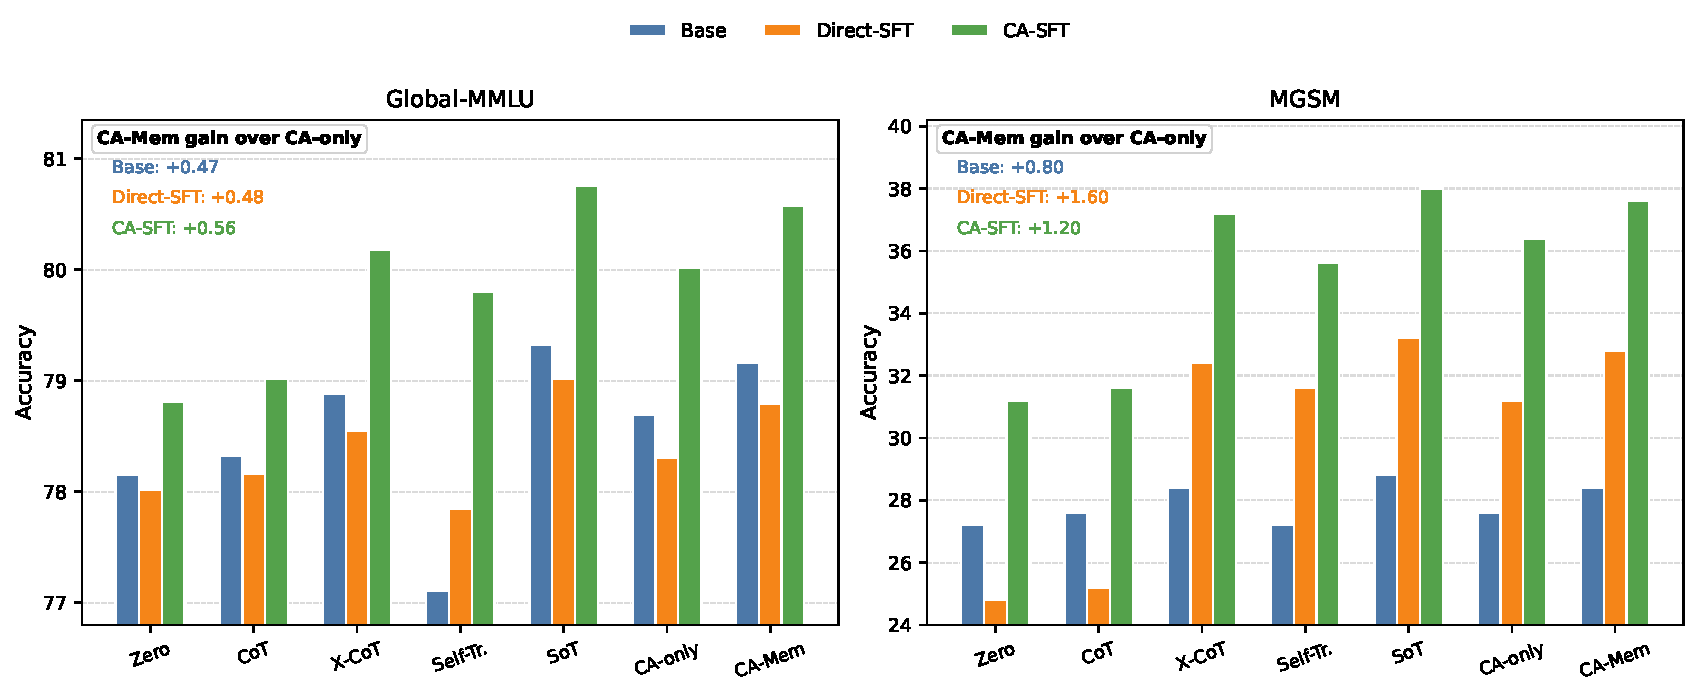
\includegraphics[width=0.98\linewidth]{figures/english_results_bars.pdf}
\caption{English results on Global-MMLU and MGSM. Each subplot compares prompting, concept-anchored, and memory-augmented methods across Base, Direct-SFT, and CA-SFT settings. Numbers above the CA-Mem bars indicate the absolute gain over CA-only.}
\label{fig:english_results}
\end{figure*}

CA-Mem also improves over CA-only in English, but the gains are smaller than in low-resource languages. This is consistent with the hypothesis that English inputs already activate internal concept knowledge more reliably, leaving less room for concept routing improvements.

\subsection{Memory Injection Breakdown}
Table~\ref{tab:memory_injected} reports the accuracy breakdown by memory-injection status.
\begin{table*}[t]
\centering
\scriptsize
\setlength{\tabcolsep}{3pt}
\renewcommand{\arraystretch}{0.95}
\begin{tabular*}{\textwidth}{@{\extracolsep{\fill}} l r r r r r r}
\hline
Group & \#Examples & CA-only Correct & CA-Mem Correct & CA-only Acc. & CA-Mem Acc. & Gain \\
\hline
Memory injected & 28,667 & 18,467 & 21,488 & 64.42 & 74.96 & +10.54 \\
No-memory fallback & 41,543 & 25,018 & 25,018 & 60.22 & 60.22 & +0.00 \\
Total & 70,210 & 43,485 & 46,506 & 61.94 & 66.24 & +4.30 \\
\hline
\end{tabular*}
\caption{Accuracy breakdown by memory-injection status on Global-MMLU with CA-SFT.}
\label{tab:memory_injected}
\end{table*}

At the development-selected threshold $\gamma=0.8$, 28,667 out of 70,210 Global-MMLU test examples receive memory injection, corresponding to 40.83\% of the test set. Table~\ref{tab:memory_injected} shows that the overall gain is concentrated in this high-confidence memory-injected subset. On the memory-injected examples, CA-Mem improves over CA-only by 10.54 points, whereas fallback cases remain identical to CA-only by construction.

\subsection{Cross-model Family Generalization}
This subsection examines whether the CA-Mem gains observed for the main model also transfer to other model families with different multilingual capabilities.
Table~\ref{tab:cross_model} reports cross-model generalization across three model families.

\begin{table*}[t]
\centering
\scriptsize
\setlength{\tabcolsep}{3pt}
\renewcommand{\arraystretch}{0.95}
\begin{tabular*}{\textwidth}{@{\extracolsep{\fill}} c l c c c c c c}
\hline
Model & Method & bn & sw & te & ne & hi & Avg. \\
\hline
 & Zero-shot & 40.56 & 41.61 & 39.14 & 41.63 & 45.80 & 41.75 \\
\raisebox{-0.5\baselineskip}[0pt][0pt]{Llama-3.1-8B-Instruct} & CoT & 39.62 & 38.97 & 19.62 & 39.04 & 45.52 & 36.55 \\
 & CA-only & 44.99 & 43.25 & 42.19 & 44.18 & 48.00 & 44.52 \\
 & CA-Mem & \textbf{48.07} & \textbf{46.42} & \textbf{45.84} & \textbf{47.30} & \textbf{50.86} & \textbf{47.70} \\
\hline
 & Zero-shot & 53.30 & 40.54 & 50.30 & 51.61 & 55.24 & 50.20 \\
\raisebox{-0.5\baselineskip}[0pt][0pt]{Ministral-3-8B-Instruct-2512} & CoT & 56.54 & 38.77 & 52.51 & 54.32 & 60.16 & 52.46 \\
 & CA-only & 56.87 & 45.23 & 55.39 & 56.27 & 59.27 & 54.61 \\
 & CA-Mem & \textbf{60.31} & \textbf{49.02} & \textbf{58.56} & \textbf{59.61} & \textbf{62.18} & \textbf{57.94} \\
\hline
 & Zero-shot & 58.64 & 54.75 & 58.90 & 59.59 & 61.34 & 58.64 \\
\raisebox{-0.5\baselineskip}[0pt][0pt]{Gemma-3-12B-it} & CoT & 59.98 & 56.37 & 60.13 & 60.45 & 61.73 & 59.73 \\
 & CA-only & 60.85 & 56.57 & 61.73 & 60.82 & 62.77 & 60.55 \\
 & CA-Mem & \textbf{63.20} & \textbf{59.05} & \textbf{63.88} & \textbf{63.14} & \textbf{64.85} & \textbf{62.82} \\
\hline
\end{tabular*}
\caption{Cross-model family generalization on Global-MMLU. CA-Mem denotes CA-only with concept usage memory.}
\label{tab:cross_model}
\end{table*}

Table~\ref{tab:cross_model} shows that CA-Mem generalizes consistently across all three model families. Relative to CA-only, the average gain is +3.18 for Llama-3.1-8B-Instruct, +3.33 for Ministral-3-8B-Instruct-2512, and +2.27 for Gemma-3-12B-it. The improvement is also broad-based across languages rather than concentrated in a single split: every model family shows positive gains on bn, sw, te, ne, and hi. Notably, the Llama-3.1-8B results also show that CoT is relatively weak compared with concept-anchored variants. This pattern supports our motivation that simply eliciting longer reasoning chains does not necessarily correct the initial cross-lingual concept routing error; when the initial concept is misactivated, CoT can elaborate an incorrect reasoning path rather than recover the intended knowledge. The corresponding radar visualization is shown in Figure~\ref{fig:cross_model_radar} in the main text.

\section{Additional Validation and Safety Analysis}
\label{sec:app_additional_validation}
This section collects validation analyses that are not part of the main result tables: raw-memory baselines, development-set threshold selection, memory safety checks, and manual failure analysis.

\subsection{Statistical Reliability}
\label{sec:app_statistical_reliability}

We estimate 95\% confidence intervals with paired bootstrap resampling over evaluation examples. For each comparison, we resample examples with replacement, recompute the aggregate metric, and report the distribution of paired score differences. Global-MMLU and MGSM use macro-average differences, while INCLUDE uses weighted-average differences. We report two-sided paired bootstrap $p$-values.

Table~\ref{tab:bootstrap_ci} shows that the main Global-MMLU and INCLUDE improvements are statistically reliable across comparisons. MGSM exhibits wider confidence intervals due to its smaller evaluation size; the gain over CA-only is positive but marginal, while comparisons against SoT and Self-Translate remain statistically reliable.

\begin{table*}[t]
\centering
\scriptsize
\setlength{\tabcolsep}{3pt}
\renewcommand{\arraystretch}{0.95}
\begin{tabular*}{\textwidth}{@{\extracolsep{\fill}} l l l c c c}
\hline
Benchmark & Metric & Comparison & Diff. & 95\% CI & $p$-value \\
\hline
Global-MMLU & Macro Avg. & CA-Mem vs. CA-only & +4.30 & [+3.98, +4.64] & <0.001 \\
Global-MMLU & Macro Avg. & CA-Mem vs. SoT & +5.02 & [+4.67, +5.36] & <0.001 \\
Global-MMLU & Macro Avg. & CA-Mem vs. Self-Translate & +4.57 & [+4.24, +4.91] & <0.001 \\
INCLUDE & Weighted Avg. & CA-Mem vs. CA-only & +4.20 & [+2.29, +6.07] & <0.001 \\
INCLUDE & Weighted Avg. & CA-Mem vs. SoT & +4.75 & [+2.85, +6.67] & <0.001 \\
INCLUDE & Weighted Avg. & CA-Mem vs. Self-Translate & +5.74 & [+3.78, +7.75] & <0.001 \\
MGSM & Macro Avg. & CA-Mem vs. CA-only & +3.07 & [-0.13, +6.27] & 0.060 \\
MGSM & Macro Avg. & CA-Mem vs. SoT & +4.00 & [+0.80, +7.20] & 0.016 \\
MGSM & Macro Avg. & CA-Mem vs. Self-Translate & +5.73 & [+2.40, +8.93] & <0.001 \\
\hline
\end{tabular*}
\caption{Paired bootstrap confidence intervals for key CA-SFT comparisons. Global-MMLU and MGSM use macro-average differences, while INCLUDE uses weighted-average differences. We report two-sided paired bootstrap $p$-values.}
\label{tab:bootstrap_ci}
\end{table*}

\subsection{Raw Memory Baselines}
Table~\ref{tab:raw_memory_baselines} reports the Global-MMLU CA-SFT raw-memory baseline protocol.
All methods use the same CA-SFT checkpoint, the same retrieval encoder, Top-1 retrieval, the same retrieval threshold, the same fallback behavior, and temperature 0.
The raw QA and raw trajectory memory variants are answer-sanitized before retrieval and do not expose gold answers, answer labels, correct option text, or answer-bearing shortcuts.

\begin{table*}[!t]
\centering
\scriptsize
\setlength{\tabcolsep}{3pt}
\renewcommand{\arraystretch}{0.95}
\resizebox{\textwidth}{!}{%
\begin{tabular}{l l l c c c c c c}
\hline
Method & Retrieval Key & Retrieved Content & bn & sw & te & ne & hi & Macro Avg. \\
\hline
CA-only & - & - & 63.61 & 60.28 & 58.05 & 61.71 & 66.03 & 61.94 \\
Raw QA Memory & English question & sanitized raw QA memory & 64.58 & 61.50 & 59.32 & 63.18 & 67.45 & 63.21 \\
Raw Trajectory Memory & English question & sanitized raw solving trajectory & 65.38 & 62.36 & 60.14 & 64.07 & 68.21 & 64.03 \\
Raw QA + Concept Key & subject + generated concept + generated description & sanitized raw QA memory & 65.72 & 62.91 & 60.61 & 64.52 & 68.67 & 64.49 \\
CA-Mem & subject + generated concept + generated description & curated concept usage memory & \textbf{67.73} & \textbf{64.63} & \textbf{62.23} & \textbf{66.20} & \textbf{70.40} & \textbf{66.24} \\
\hline
\end{tabular}
}
\caption{Raw-memory baselines on Global-MMLU with CA-SFT. All methods use the same CA-SFT checkpoint, retrieval encoder, Top-1 retrieval, threshold, fallback behavior, and decoding setting. Raw QA and raw trajectory memories are answer-sanitized before retrieval.}
\label{tab:raw_memory_baselines}
\end{table*}

The raw-memory variants improve over CA-only, indicating that source-side examples and trajectories contain transferable signals. However, both sanitized raw QA memory and sanitized raw trajectory memory remain below CA-Mem. Raw QA + Concept Key further improves over English-question retrieval, showing that concept-normalized retrieval keys are beneficial even for raw memory. The best performance is achieved by CA-Mem, suggesting that curated procedural usage summaries provide less noisy and more actionable guidance than raw retrieved context.

\subsection{Development-Set Threshold Selection}
The default retrieval threshold $\gamma=0.8$ is selected on a held-out development split.
This development split is not used for CA-SFT training or memory construction.
After selecting $\gamma=0.8$, we keep this value fixed for all test evaluations.

\begin{table}[!htbp]
\centering
\scriptsize
\setlength{\tabcolsep}{5pt}
\renewcommand{\arraystretch}{0.95}
\begin{tabular}{l c c}
\hline
$\gamma$ & Dev Coverage & Dev Accuracy \\
\hline
0.5 & 75.80\% & 64.35 \\
0.6 & 65.20\% & 65.02 \\
0.7 & 53.10\% & 65.71 \\
0.8 & 41.40\% & \textbf{66.08} \\
0.9 & 22.30\% & 65.54 \\
\hline
\end{tabular}
\caption{Development-set threshold selection. The threshold $\gamma=0.8$ achieves the best development accuracy and is fixed before all test evaluations. Coverage denotes the percentage of examples receiving memory injection.}
\label{tab:dev_threshold_selection}
\end{table}

As $\gamma$ increases, memory coverage decreases while memory precision improves. The development results peak at $\gamma=0.8$, which provides the best balance between accuracy and coverage. We therefore fix $\gamma=0.8$ before test evaluation rather than selecting the threshold on test results.

\subsection{Leakage Control and Memory Safety Audit}
Table~\ref{tab:leakage_safety_audit} summarizes the leakage-control and memory-safety audit.

\begin{table*}[!t]
\centering
\scriptsize
\setlength{\tabcolsep}{4pt}
\renewcommand{\arraystretch}{0.95}
\resizebox{\textwidth}{!}{%
\begin{tabular}{l l l}
\hline
Risk & Control / Audit Check & Status \\
\hline
Source--test overlap & Remove exact, normalized, and answer-equivalent source--test duplicates before SFT and memory construction & Filtered \\
Answer leakage & Exclude gold labels, answer labels, correct-option text, and answer-bearing shortcuts from memory nodes & Controlled \\
Raw-instance memorization & Exclude source questions, option text, and raw QA content; retain only sanitized concept descriptions and usage summaries & Controlled \\
Test-time contamination & Freeze the memory bank before evaluation; test examples only perform read-only retrieval & Controlled \\
\hline
\end{tabular}
}
\caption{Leakage-control and memory-safety audit.}
\label{tab:leakage_safety_audit}
\end{table*}

The following memory-node examples show only sanitized reusable fields. They omit source questions, options, answer labels, gold answers, and correct option text.

\begin{quote}\small
\textbf{Subject:} law\\
\textbf{Concept:} Obscenity regulation\\
\textbf{Description:} Government may regulate obscene material, but protected speech boundaries require applying the relevant doctrinal criteria rather than treating all adult content as automatically unprotected.\\
\textbf{trigger\_invariants:} Activate this concept when a legal question concerns restrictions on allegedly obscene expression, public distribution, private access, or the boundary between protected and unprotected speech.\\
\textbf{decision\_rules:} Identify whether the rule targets obscene material under the governing doctrinal test, then check the context of access, distribution, and statutory scope before deciding whether regulation is permissible.\\
\textbf{negative\_error\_boundaries:} Do not assume that any adult-oriented material is automatically regulable; avoid collapsing private or limited-access contexts into public distribution.
\end{quote}

\begin{quote}\small
\textbf{Subject:} biology\\
\textbf{Concept:} Endosymbiotic theory\\
\textbf{Description:} The endosymbiotic theory explains the origin of mitochondria and chloroplasts through ancestral symbiotic relationships between cells.\\
\textbf{trigger\_invariants:} Activate this concept when a biology question asks about organelle origins, mitochondria, chloroplasts, bacterial-like features, membranes, DNA, or evolutionary evidence for symbiosis.\\
\textbf{decision\_rules:} Compare each candidate claim against stable evidence for endosymbiosis, such as organelle autonomy, genetic material, replication patterns, and bacterial-like structural features.\\
\textbf{negative\_error\_boundaries:} Do not treat generic organelle function as evidence for origin; avoid confusing current cellular roles with evolutionary support for the theory.
\end{quote}

\subsection{Manual Failure Analysis}
We sample 100 incorrect Global-MMLU cases from the CA-SFT + CA-Mem setting, using an approximately stratified sample across bn, sw, te, ne, and hi where possible.
Each error is assigned one primary failure type: concept activation error, retrieval mismatch, insufficient procedural guidance, reasoning / execution error, or benchmark or translation ambiguity.

\begin{table}[!htbp]
\centering
\scriptsize
\setlength{\tabcolsep}{4pt}
\renewcommand{\arraystretch}{0.95}
\begin{tabular}{l c c}
\hline
Failure Type & Count & Proportion \\
\hline
Concept activation error & 34 & 34\% \\
Retrieval mismatch & 12 & 12\% \\
Insufficient procedural guidance & 18 & 18\% \\
Reasoning / execution error & 28 & 28\% \\
Benchmark or translation ambiguity & 8 & 8\% \\
Total & 100 & 100\% \\
\hline
\end{tabular}
\caption{Manual failure analysis of 100 randomly sampled CA-Mem errors on Global-MMLU under CA-SFT.}
\label{tab:manual_failure_analysis}
\end{table}

The largest remaining failure source is concept activation error, where the generated English concept is overly broad or misaligned with the question. Reasoning and execution errors are also frequent, especially for questions requiring multi-step computation, fine-grained option comparison, or exact symbolic manipulation. Retrieval mismatch accounts for a smaller portion of failures, suggesting that gated concept-based retrieval usually avoids injecting unrelated memory once the upstream concept is correctly activated. These results indicate that CA-Mem primarily depends on reliable concept activation and final reasoning quality, rather than retrieval alone.

\section{Prediction Flip Analysis}
\label{sec:app_prediction_flip}
\label{sec:appendix_flip}
This section provides the per-language breakdown of prediction flips between CA-only and CA-Mem in Table~\ref{tab:prediction_flip}.
A prediction flip analysis further shows that CA-Mem rescues 3,251 CA-only errors while introducing only 230 new errors, yielding a net gain of 3,021 additional correct predictions.

\begin{table}[!htbp]
\centering
\scriptsize
\setlength{\tabcolsep}{2pt}
\renewcommand{\arraystretch}{0.94}
\begin{tabular}{l r r r r r r r}
\hline
Lang & Both C. & Resc. & Hurt & Both W. & Net & Resc. & Hurt \\
\hline
bn & 8,890 & 621 & 42 & 4,489 & +579 & 12.16 & 0.47 \\
sw & 8,417 & 658 & 48 & 4,919 & +610 & 11.80 & 0.57 \\
te & 8,097 & 641 & 54 & 5,250 & +587 & 10.88 & 0.66 \\
ne & 8,619 & 677 & 46 & 4,700 & +631 & 12.58 & 0.53 \\
hi & 9,232 & 654 & 40 & 4,116 & +614 & 13.71 & 0.43 \\
Total & 43,255 & 3,251 & 230 & 23,474 & +3,021 & 12.16 & 0.53 \\
\hline
\end{tabular}
\caption{Prediction flip analysis of CA-Mem relative to CA-only on Global-MMLU with CA-SFT.}
\label{tab:prediction_flip}
\end{table}
\FloatBarrier

\section{Qualitative Case Studies}
\label{sec:appendix_cases}

This section presents answer-sanitized qualitative cases selected from prediction flips and retrieval diagnostics. To avoid benchmark leakage, we omit gold labels, option texts, and direct answer-bearing content. We include success, failure, and contrastive cases to illustrate when concept anchoring and concept usage memory help, and when upstream concept errors or retrieval mismatch still limit CA-Mem.

\begin{table*}[!htbp]
\centering
\scriptsize
\setlength{\tabcolsep}{3pt}
\renewcommand{\arraystretch}{0.95}
\caption{Summary of answer-sanitized qualitative cases.}
\label{tab:case_summary}
\resizebox{\textwidth}{!}{%
\begin{tabular}{l l l l}
\hline
Case & Type & Subject & Main Insight \\
\hline
A & Success & law & Memory repairs concept usage \\
B & Success & biology & Anchoring prevents retrieval drift \\
C & Failure & economics & Wrong concept activates wrong memory frame \\
D & Contrastive failure & physics & Non-anchored retrieval drifts cross-domain \\
\hline
\end{tabular}%
}
\end{table*}

\subsection{Case A: Memory Repairs Concept Usage}
\noindent\textbf{Language / Subject:} bn / law\\
\textbf{Case Type:} Success --- CA-only wrong, CA-Mem correct\\
\textbf{Question gist:} The question concerns whether a motel owner can be prosecuted for showing adult films privately inside motel rooms, under a statute that prohibits obscene films in places open to the public.\\
\textbf{Activated concept:} Obscenity regulation\\
\textbf{Retrieved memory:}

The retrieved memory is shown in sanitized form and does not include source question text, option text, or answer labels.

\begin{quote}\small
\textbf{Concept:} Obscenity regulation \\
\textbf{Subject:} law \\
\textbf{Description:} Government may ban obscene material, but ordinary speech is protected unless it meets strict obscenity criteria. \\
\textbf{Sanitized usage cue:} Before applying a general obscenity regulation, check the doctrinal boundary of the rule; distinguish public distribution from private or limited-access contexts.
\end{quote}

\noindent\textbf{Outcome:} CA-only predicts incorrectly, whereas CA-Mem uses the retrieved procedural cue and answers correctly.\\
\textbf{Interpretation:} This case shows that CA-only can activate the right concept but still apply it too broadly. The model correctly identifies the relevant doctrine as \textit{Obscenity regulation}, but CA-only treats the general power to regulate obscene material as sufficient for upholding the prosecution. CA-Mem retrieves a memory node that does not contain an answer cue, but instead reminds the model to check the boundary condition of the doctrine, especially the distinction between public distribution and private or limited-access viewing. This procedural cue repairs the concept-usage error and flips the final prediction to the correct answer.\\
\textbf{Takeaway:} CA-only helps the model identify what concept is relevant, while CA-Mem helps the model determine how to apply that concept under the specific constraints of the question.

\subsection{Declarative vs. Procedural Memory Contrast}
\label{sec:app_declarative_procedural_contrast}

To further clarify the distinction between declarative and procedural memory, we revisit Case A under the same answer-sanitized diagnostic setting. The retrieved \textit{description} provides a general definition of the activated concept, whereas the \textit{usage summary} specifies how the concept should be applied under boundary conditions.

\begin{quote}\small
\textbf{Declarative description only:} Government may ban obscene material, but ordinary speech is protected unless it meets strict obscenity criteria.

\textbf{Procedural usage summary:} Before applying a general obscenity regulation, check the doctrinal boundary of the rule; distinguish public distribution from private or limited-access contexts.
\end{quote}

The description-only cue identifies the broad legal doctrine but does not specify which contextual distinction should control the decision. In contrast, the procedural usage summary highlights the relevant boundary condition and instructs the model to avoid over-applying the general rule. This illustrates why concept usage memory is not merely a declarative concept definition: it provides an application procedure for using the activated concept under task-specific constraints. This qualitative pattern is consistent with the memory-content ablation in Table~\ref{tab:ablation_main}, where \textit{Usage Summary Only} yields a larger gain than \textit{Description Only}.

\subsection{Case B: Concept Anchoring Prevents Cross-Lingual Retrieval Drift}
\noindent\textbf{Language / Subject:} sw / biology\\
\textbf{Case Type:} Success --- low-resource retrieval drift corrected by concept anchoring\\
\textbf{Question gist:} The item asks which statement does not support the endosymbiotic theory of the origin of mitochondria and chloroplasts.\\
\textbf{Activated concept:} Endosymbiotic theory\\
\textbf{Retrieval comparison:}

\begin{quote}\small
\textbf{Without anchoring:} \textit{Prejudgment attachment} (law; mismatched retrieval) \\
\textbf{With concept anchoring:} \textit{Endosymbiotic theory} (biology; aligned retrieval)
\end{quote}

\noindent\textbf{Outcome:} Direct raw-question retrieval drifts to an unrelated law memory, whereas concept-anchored retrieval returns the aligned biology memory and yields the correct prediction.\\
\textbf{Interpretation:} This case illustrates why CA-Mem does not retrieve memory directly with the raw low-resource-language question. The drift from a biology problem to an unrelated law memory indicates a representation mismatch between the low-resource surface form and the English concept-level memory bank. After anchoring through the generated concept and description, retrieval becomes concept-aligned and the final prediction becomes correct.\\
\textbf{Takeaway:} Concept anchoring stabilizes cross-lingual retrieval. It converts a noisy low-resource-language question into a high-resource concept key that can reliably access the intended memory node.

\subsection{Case C: Wrong Concept Activation Leads Memory to the Wrong Frame}
\noindent\textbf{Language / Subject:} bn / economics\\
\textbf{Case Type:} Failure --- generated concept is wrong\\
\textbf{Question gist:} The question asks how money demand changes when nominal GDP increases.\\
\textbf{Activated concept:} Interest rate effect\\
\textbf{Error source:} Concept activation error.\\
\textbf{Retrieved memory:}

\begin{quote}\small
\textbf{Concept:} Interest rate effect \\
\textbf{Subject:} economics \\
\textbf{Description:} The interest rate effect is the change in money demand caused by changes in the interest rate.
\end{quote}

\noindent\textbf{Outcome:} CA-only and CA-Mem both remain incorrect because retrieval follows the mistaken concept anchor instead of the intended economic mechanism.\\
\textbf{Interpretation:} This failure occurs at the concept activation stage. The underlying question is about nominal GDP and transaction demand for money, not primarily about an interest-rate shift. Because retrieval is conditioned on the generated concept, CA-Mem faithfully follows the wrong conceptual frame and cannot recover the answer. Retrieval therefore reinforces the mistaken reasoning path instead of redirecting it.\\
\textbf{Takeaway:} CA-Mem is not an oracle retriever. Its effectiveness depends on the quality of upstream concept activation. When the generated concept is wrong, memory can reinforce the wrong reasoning frame instead of correcting it.

\subsection{Case D: Retrieval Drift without Concept Anchoring}
\noindent\textbf{Language / Subject:} bn / physics\\
\textbf{Case Type:} Contrastive failure --- non-anchored retrieval drift\\
\textbf{Question gist:} The item asks for the order of element layers formed around a star as stellar evolution progresses, starting from the outer layer.\\
\textbf{Activated concept:} Not applicable in this non-anchored contrast.\\
\textbf{Non-anchored retrieval result:}

\begin{quote}\small
\textbf{Non-anchored retrieved memory:} \textit{Ignorance of refutation} (philosophy; mismatched retrieval)
\end{quote}

\noindent\textbf{Outcome:} Retrieval drifts to an irrelevant philosophy memory and fails before concept-aligned reasoning can be established. This is a contrastive failure case for non-anchored retrieval, not the final CA-Mem configuration.\\
\textbf{Interpretation:} In this case, the underlying physics question concerns stellar nucleosynthesis and the sequence of element layers formed during stellar evolution. Without concept anchoring, retrieval can still return an unrelated philosophy memory that is procedurally unhelpful for the target concept. We therefore present this case as a retrieval-boundary contrast rather than as a failure of the final anchored CA-Mem system.\\
\textbf{Takeaway:} CA-Mem requires both a useful concept anchor and precise memory retrieval. The anchored subject + generated concept + generated description query helps prevent this kind of cross-domain retrieval drift.


\FloatBarrier
\end{document}
